 \chapter{ در ساختار دسترسی رادیویی ابری‌ادبیات و پیشینه ی تحقیق}
 \section{مقدمه}
 شبکه های دسترسی رادیویی ابری، می تواند ساختار جدیدی برای نسل بعدی سیستمهای مخابراتی سلولی باشد. در این ساختار، پردازش های بخش باند پایه از ایستگاه پایه \LTRfootnote{BS}، به واحد کنترل \LTRfootnote{CU} در داخل ابر \LTRfootnote{cloud} منتقل می گردد. ایستگاه باند پایه که به عنوان واحد رادیویی \LTRfootnote{RRH} عمل می کند، توسط لینک \lr{fronthaul}، به واحد کنترل متصل می گردد. لینک \lr{fronthaul}، اطلاعاتی در مورد سیگنالهای باند پایه که در حالت فراسو از واحد رادیویی به واحد کنترل و در حالت فروسو به صورت برعکس ، منتقل می کند. بدلیل محدودیت در ظرفیت لینک \lr{fronthaul}،\cite{fc} اطلاعات قبل از عبور از این لینک، کوانتیزه می گردد.
 %%%%%%%%%%%%%%%%%%%%%%%%%%
 
 
در حال حاضر بسیاری از تحقیقات در زمینه ی \lr{5G} در مورد سیستم های \lr{MIMO} است که در زیرساخت \lr{C-RAN} می باشد.
در این فصل، برخی از نتایج ارائه شده مرتبط با شبکه های دسترسی رادیویی ابری در لینک فروسو و  فراسو بیان می گردد.
\section{لینک فروسو}
در این قسمت، سیستمهای  \lr{MIMO C-RAN} در حالت فروسو مورد بررسی قرار می گیرد. در حالت فروسو،  واحد کنترل، پردازش اطلاعات پیام را با عملکرد کدگذاری کانال و پیش کد گذاری \LTRfootnote{precoding} مدیریت می نماید.
\subsection{مدل سیستم اول}
سیگنال پیش کدگذاری شده ی باند پایه در واحد کنترل، فشرده گشته و توسط لینک ارتباطی \lr{fronthaul} که دارای ظرفیت محدود است \cite{fc2}، به واحد رادیویی منتقل می گردد.
هر واحد رادیویی، از لینک \lr{fronthaul} سیگنالی را که دارای نویز کوانتیزاسیون است، دریافت می کند؛ سپس با اعمال \lr{pulse shaping}، سیگنال را به فرکانس بالاتر منتقل کرده و از طریق کانال بدون سیم به کاربران ارسال می نماید.
\begin{figure}[H]
  \centering
    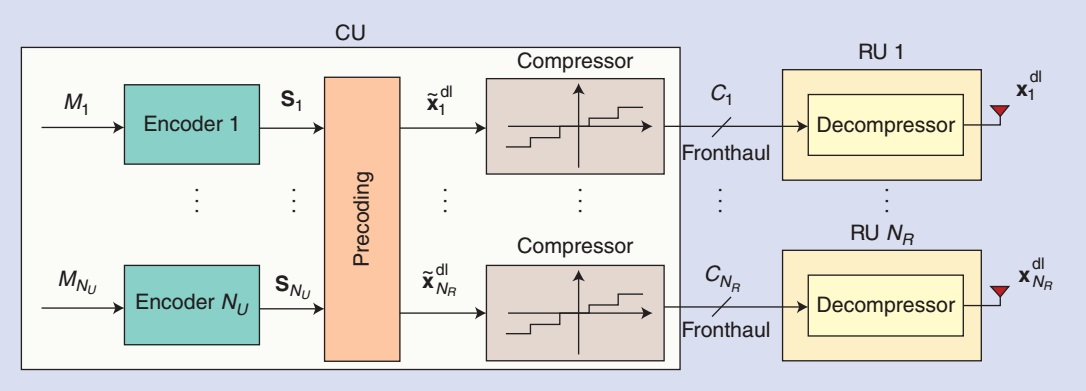
\includegraphics[width=\linewidth, height=6cm]{dl}
  \caption{مسیر انتقال پیام در لینک فروسو \cite{Fronthaul}.}
  \label{fig:dl}
\end{figure}
بلوک دیاگرام مدل سیستم اول
در شکل \ref{fig:dl} نشان شده است. 
در اینجا، $N_U$ کاربر قرار دارند که توسط $N_R$ واحد رادیویی سرویس دهی می شوند.


برای بدست آوردن سیگنال 
$\tilde{\boldsymbol{x}}^{dl}$ ،
واحد کنترل، سیگنال پیام را به صورت مجزا برای هر کاربر کدگذاری می کند.  با  اعمال این فرآیند،  سمبلهای $\boldsymbol{s}=[s_1;...;s_{N_U}]$  بدست می آید که $s_k$ نشان دهنده ی سمبل $k$ امین کاربر می باشد. 
سیگنال پیش کدگذاری شده ی
$\tilde{\boldsymbol{x}}^{dl} $
که توسط واحد کنترل تولید می گردد به این صورت بیان می شود:
\begin{equation}\label{wp}
 \tilde{\boldsymbol{x}}^{dl} = \boldsymbol{W}\boldsymbol{P}^{\frac{1}{2}} \boldsymbol{s},
\end{equation}
که 
 \begin{equation}
\tilde{\boldsymbol{x}}^{dl} = [\tilde{x}_{1}^{dl}; ... ; \tilde{x}_{N_R}^{dl}] 
 \end{equation}
 در رابطه ی  \eqref{wp}، $\boldsymbol{W}$، ماتریس پیش کدگذاری شده با ابعاد $N_R \times N_U$ می باشد و $\boldsymbol{W} = [\boldsymbol{w_1},..., \boldsymbol{w_{N_{U}}}]$ است. علاوه بر این، 
 $\boldsymbol{P}^{\frac{1}{2}} = diag(\sqrt{p_1},...,\sqrt{p_{N_U}})$ 
 ماتریس توان است.
حال سیگنال فشرده شده ی دریافتی توسط واحد رادیویی به صورت زیر بدست می آید:
\begin{equation}
\label{eq_pow1}
 {\boldsymbol{x}}^{dl} = \tilde{\boldsymbol{x}}^{dl} + \boldsymbol{Q},
\end{equation}
که در اینجا $\boldsymbol{Q} = \left[ q_1,\ldots,q_{N_R}\right]^T$، بردار نویز کوانتیزاسیون تولید شده به دلیل فشرده سازی بعد از پیش کدگذاری در واحد کنترل می باشد که دارای توزیع 
 $ \forall i  \quad  q_i\backsim \mathcal{N}(0,\sigma_{q_i^2}) $ 
 می باشد.
%%%%%%%%%%%%%%%%%%5
سیگنال دریافتی توسط $j$ امین کاربر به صورت $y_j$ نمایش داده می شود.
\begin{equation}
{y}_j = \boldsymbol{H}_j \boldsymbol{x}^{dl}+ z_j
\end{equation}
 $\boldsymbol{H}_j $
  بردار کانال کاربر $j$ام می باشد 
  که دارای ابعاد
 $1 \times N_R$ 
 است. همچنین
    $z_j$ نویز گوسی 
 $z_j \backsim \mathcal{N}(0,1) $ می باشد.
توان ارسالی از $i$ امین واحد رادیویی از رابطه ی زیر بدست می آید:
\begin{equation}\label{pr}
P_i (\boldsymbol{W},\sigma_q) = \frac{1}{T} E[{||{x_i}||}^2] = trace(\boldsymbol{w_i}\boldsymbol{P}^{\frac{1}{2}}(\boldsymbol{P}^H)^{ \frac{1}{2}}\boldsymbol{w_i}^H + \sigma_{q_i}^2 \boldsymbol{I})
\end{equation}
که در اینجا 
$T=1$
 می باشد.
همچنین 
$\sigma_{q_i}^2$
واریانس نویز کوانتیزاسیون است.
با توجه به رابطه ی \eqref{pr}
ظرفیت لینک \lr{fronthaul} از واحد کنترل به  $i$ امین واحد رادیویی 
از رابطه ی زیر بدست می آید:
\begin{equation}
C_i(\boldsymbol{W},\sigma_{q_i}) = \log det(\boldsymbol{w_i}\boldsymbol{P}^{\frac{1}{2}}(\boldsymbol{P}^H)^{ \frac{1}{2}}\boldsymbol{w_i}^H + \sigma_{q_i}^2 \boldsymbol{I}) - \log (\sigma_{q_i}^2)
\end{equation}
%%%%%%%%%%%%%%%%%%%%%%%%%%%%%5%%%%%%%%%
برای بدست آوردن نرخ قابل دسترس $j$ امین کاربر از فرمول زیر استفاده می گردد:

\begin{equation}
\boldsymbol{R}_j (\boldsymbol{W},\boldsymbol{\sigma_q})=I(s_j;y_j) 
\end{equation}
که در اینجا 
$I$
همان اطلاعات متقابل است.


 در این تحقیقات، مجموع نرخ های قابل دسترس براساس محدودیت ظرفیت لینک \lr{fronthaul} و محدودیت توان هر واحد رادیویی، بیشینه می گردد:
\begin{equation}
\begin{aligned}
\max\limits_{\boldsymbol{W},\boldsymbol{\sigma_q}}   \quad &   \sum_j R_j(\boldsymbol{W},\boldsymbol{\sigma_q})\\
\text{\lr{subject to}} \quad  & \bar{P}_i(\boldsymbol{W}, \sigma_q) \leq P_{max} \ \  \forall i \\
&C_i(\boldsymbol{W},\sigma_q)\leq C^{th}  \ \ \forall i \\
\end{aligned}
\end{equation}

 
%%%%%%%%%%%%%%%%%%%%%%%%%%%%%%%%%%%%%%%%%%%%%%%%%%%%%%%%%%%%%%%%%
در اینجا می خواهیم مجموع نرخ ها با محدودیت بیان شده را بیشینه کنیم. برای حل این مسائل از الگوریتم تکرار شونده و ضرایب لاگرانژ که در فصل بعدی ارائه می گردد، استفاده می شود \cite{ul_dl,ulSimeone, Fronthaul, precodSimeone}.

%%%%%%%%%%%%%%%%%%%%%%%%%%%%%%%%%%%%%%%%%%%%%%%%%%%%%%%%%%%
\subsection{مدل سیستم دوم}
در این بخش، مدل سیستم دومی را برای ساختار \lr{MIMO C-RAN} بررسی می کنیم. 


فرض بر این است که کاربران و \lr{RRH}ها، به 
 $S$
 تا خوشه تقسیم شده اند که $v$ امین خوشه،
 دارای $R_v$ تا \lr{RRH} است که ${D}_v$ تا کاربر را سرویس دهی می کنند.
همچنین  $r_{(s,n)}$
 نشان دهنده ی $n$ امین واحد رادیویی در $s$ امین خوشه می باشد  و به همین صورت $d_{(s,k)}$
 نشان دهنده ی $k$ امین کاربر در $s$ امین خوشه است.

 \begin{figure}[H]
  \centering
    \includegraphics[scale=1]{mimoCRAN}
  \caption{ساختار \lr{MIMO C-RAN} \cite{EEcluster}.}
  \label{fig:mimoC-RAN}
\end{figure}
در این قسمت، بردار سیگنال دریافتی کاربران در $s$ امین خوشه، به صورت زیر نوشته می شود:
\begin{equation} \label{sg}
\boldsymbol{y}_{\mathcal{D}_s} = \sum_{v=1}^S \boldsymbol{H}^H_{\mathcal{R}_v,\mathcal{D}_s}\boldsymbol{W}_{R_v, {D}_v}\boldsymbol{P}_{{D}_v}^\frac{1}{2}\boldsymbol{x}_{\mathcal{D}_v}+ \boldsymbol{z}_{\mathcal{D}_s},
\end{equation}
که در اینجا 
$\boldsymbol{x}_{ \mathcal{D}_v} = [x_{ d_{(v,1)}},..., x_{ d_{(v,D_v)}}]^T \in C^{ \mathcal{D}_v \times 1} $ 
بردار سمبل ارسالی واحد رادیویی از $t$ امین خوشه می باشد.

%%%%%%%%%%%%%%%%%%%%%%%%%%%%%%%%%%%%%%%%%%%%%%%%%%%%%%%
  $\boldsymbol{W}_{R_v, \boldsymbol{D}_v} = [\boldsymbol{w}_{ R_v,d_{(v,1)}},..., \boldsymbol{w}_{R_v, d_{(v,D_v)}}]^T \in C^{ R_v \times D_v} $ 
  ماتریس پیش کدگذاری اعمال شده در خوشه ی $v$ ام می باشد.
 علاوه بر این، $z_{D_s}$ نویز گوسی جمع شونده است که به صورت 
 $\boldsymbol{z_{\mathcal{D}_s}} \backsim \mathcal{N}(0,N_0\boldsymbol{I}_{{D}_s})$ 
و دارای توان $N_0$
می باشد.
همچنین $\boldsymbol{H}_{R_v,D_s}$ بردار کانال از واحدهای رادیویی دسته ی $R_v$ به کاربر دسته ی $D_s$ می باشد که این بردار را می توان به صورت زیر نوشت.
 $\boldsymbol{H}_{\mathcal{R}_v,\mathcal{D}_s}=\left[\boldsymbol{h}_{\mathcal{R}_v,d_{(s,1)}},\ldots,\boldsymbol{h}_{\mathcal{R}_v,d_{(s,\mathcal{D}_s)}}\right]^T  \in \mathbb{C}^{{R}_v\times {D}_s}$ 
 و همین طور
 بردار کانال از \lr{RRH} های خوشه ی  $v$ به $k$ امین کاربر در خوشه ی $s$ام  
 $\boldsymbol{h}_{\mathcal{R}_v,d_{(s,k)}}\in \mathbb{C}^{{R}_v}$
 به صورت زیر مدل می شود
 \begin{equation}\label{channel}
\boldsymbol{h}_{\mathcal{R}_v,d_{(s,k)}} = \boldsymbol{\beta}^\frac{1}{2}_{\mathcal{R}_v,d_{(s,k)}} \boldsymbol{g}_{\mathcal{R}_v,d_{(s,k)}},
\end{equation}
که  در اینجا $\boldsymbol{g}_{\mathcal{R}_v,d_{(s,k)}} \backsim \mathcal{N}(0,N_0\boldsymbol{I}_{\mathcal{D}_s})$ نشان دهنده ی بردار کانال محو شدگی سریع و مسطح برای کانال می باشد 
و $\boldsymbol{\beta}_{\mathcal{R}_v,d_{(s,k)}}=\text{\lr{diag}}(a_{r_{(v,1),d_{(s,k)}}},\ldots,a_{r_{(v,\mathcal{R}_v),d_{(s,k)}}})$
نشان دهنده ی محوشدگی  در مقیاس بزرگ می باشد. 
%%%%%%%%%%%%%%5
این مدل سیستم نیز شبیه به  مدل سیستم مسئله ی قبلی است با این تفاوت که در اینجا، فشرده سازی اعمال نمی گردد  $\boldsymbol{Q}_{\mathcal{R}_v} = \boldsymbol{0}$ و فرض این است که ظرفیت لینک  \lr{fronthaul} نامحدود است. 
به علاوه، در اینجا چندین خوشه باهم در نظر گرفته شده است و تداخل پیامها بین خوشه های متفاوت نیز محاسبه می شود.\newline
حال می خواهیم توان ارسالی از هر واحد رادیوی $i$ در خوشه ی $s$ به کاربران را محاسبه نمود.
\begin{equation}
\bar{p}_{r_{(s,i)}} = || \boldsymbol{w}_{r_{(s,i)},D_s}\boldsymbol{P}_{{D}_s}^\frac{1}{2}  ||^2
\end{equation} 
که در اینجا
$\boldsymbol{w}_{r_{(s,i)},D_s}$
سطر $i$ ام ماتریس $\boldsymbol{W}_{R_s, {D}_s}$
است.\newline
در حالت کلی برای بدست آوردن بردار کانال، در لینک فراسو با ارسال پایلوت، بردار کانال بدست می آید که در اینجا فرض می شود که با اندکی خطا همراه است و به این صورت بیام می گردد.
\begin{equation*}
\hat{\boldsymbol{h}}_{\mathcal{R}_v,d_{(s,k)}} = \boldsymbol{h}_{\mathcal{R}_v,d_{(s,k)}} + \Delta \boldsymbol{h}_{\mathcal{R}_v,d_{(s,k)}},
\end{equation*}

$\Delta \boldsymbol{h}_{\mathcal{R}_v,d_{(s,k)}}$
نشان دهنده ی بردار خطای تخمین زده شده است که دارای توزیع گوسی به صورت
$$\Delta \boldsymbol{h}_{\mathcal{R}_v,d_{(s,k)}}\backsim \mathcal{N}(0,\boldsymbol{\phi}_{\mathcal{R}_v,d_{(s,k)}}^2),$$
است که  داریم 
$$\boldsymbol{\phi}_{\mathcal{R}_v,d_{(s,k)}} = \text{\lr{diag}}(\phi_{r_{(v,1)},d_{(s,k)}},\ldots,\phi_{r_{(v,\mathcal{R}_v)},d_{(s,k)}}).$$
همچنین با فرض اینکه پیش کدگذاری اعمال شده از نوع \lr{MMSE} می باشد، ماتریس پیش کدگذاری از رابطه ی داده شده بدست می آید:
\begin{equation}
\boldsymbol{W}_{\mathcal{R}_s,\mathcal{D}_s} = \hat{\boldsymbol{H}}_{\mathcal{R}_s,\mathcal{D}_s}(\hat{\boldsymbol{H}}_{\mathcal{R}_s,\mathcal{D}_s}^H \hat{\boldsymbol{H}}_{\mathcal{R}_s,\mathcal{D}_s}+ \alpha \boldsymbol{I}_{{D}_s})^{-1},
\end{equation} 
 $\alpha$
  فاکتور رگولاسیون است که در صورتی که
  مقدارش صفر باشد، پیش کدگذاری
از نوع  
   \lr{ZF} 
  خواهد بود.
همچنین در صورتی که از پیش کدگذاری \lr{MRT} استفاده نماییم، ماتریس پیش کدگذاری از رابطه ی مقابل بدست می آید:
\begin{equation}
\boldsymbol{W}_{\mathcal{R}_s,\mathcal{D}_s} = \hat{\boldsymbol{H}}_{\mathcal{R}_s,\mathcal{D}_s}
\end{equation} 
همچنین این ماتریس با روشهای مختلفی قابل نرمالیزه شدن است.
حال برای فهم بیشتر، سیگنال دریافتی کاربر $d_{(s,k)}$ را نمایش می دهیم
\begin{equation}
\begin{split}
y_{d_{(s,k)}} &= \boldsymbol{h}_{\mathcal{R}_s, d_{(s,k)}}^H  \boldsymbol{w}_{\mathcal{R}_{s},d_{(s,k)}} p_{d_{(s,k)}}^\frac{1}{2}\\
&+ \underbrace{\sum_{\substack{l=1 \\ l\neq k}}^{{D}_s} \boldsymbol{h}_{\mathcal{R}_s, d_{(s,k)}}^H \boldsymbol{w}_{\mathcal{R}_{s},d_{(s,l)}}  p_{d_{(s,l)}}^\frac{1}{2}}_{\text{(\lr{intra-cluster interference})}}\\
&+\underbrace{\sum_{\substack{v=1 \\ v\neq s}}^{S} \sum_{l=1}^{{D}_s} \boldsymbol{h}_{\mathcal{R}_v, d_{(s,k)}}^H \boldsymbol{w}_{\mathcal{R}_{v},d_{(v,l)}} p_{d_{(v,l)}}^\frac{1}{2}}_{\text{(\lr{inter-cluster interference})}}\\
& +z_{d_{(s,k)}}
\end{split}
\end{equation}
%%%%%%%%%%%%%%%%%%%%%%%%%%%5
بنابراین مقدار \lr{SINR}  $k$امین کاربر در $s$امین خوشه به صورت زیر محاسبه می شود \cite{algamal, cover}؛
\begin{equation}\label{5}
\gamma_{d_{(s,k)}}= \frac{p_{d_{(s,k)}}|\boldsymbol{h}_{\mathcal{R}_s, d_{(s,k)}}^H \boldsymbol{w}_{\mathcal{R}_{s},d_{(s,k)}}|^2}{I_{d_{(s,k)}}+BN_0}.
\end{equation}
که $B$ پهنای باند کانال است و 
$I_{d_{(s,k)}}$
توان سیگنال تداخلی می باشد که از رابطه ی زیر بدست می آید؛
\begin{equation}\label{6}
\begin{split}
I_{d_{(s,k)}} &=  \underbrace{\sum_{\substack{l=1 \\ l\neq k}}^{{D}_s} |\boldsymbol{h}_{\mathcal{R}_s, d_{(s,k)}}^H \boldsymbol{w}_{\mathcal{R}_{s},d_{(s,l)}}|^2  p_{d_{(s,l)}}}_{\text{(\lr{intra-cluster interference})}}\\
&+\underbrace{\sum_{\substack{v=1 \\ v\neq s}}^{S} \sum_{l=1}^{{D}_s} |\boldsymbol{h}_{\mathcal{R}_v, d_{(s,k)}}^H \boldsymbol{w}_{\mathcal{R}_{v},d_{(v,l)}}|^2 p_{d_{(v,l)}}}_{\text{(\lr{inter-cluster interference})}}\\
\end{split}
\end{equation}

بنابراین نرخ قابل دسترسی برای کاربر $d_{(s,k)}$ به صورت زیر محاسبه می شود؛
\begin{equation}\label{e1}
\mathfrak{R}_{d_{(s,k)}} = B \log_2(1+\gamma_{d_{(s,k)}}),
\end{equation}
بازدهی انرژی نسبت مجموع نرخ های قابل دسترس به مجموع توان ارسالی می باشد که به این صورت نمایش داده می شود:
\begin{equation}\label{eta}
\eta(\boldsymbol{P}) := \frac{\sum\limits_{s=1}^{S} \sum\limits_{k=1}^{{D}_s}\mathfrak{R}_{d_{(s,k)}} }{\sum\limits_{s=1}^{S} \sum\limits_{i=1}^{{R}_s}\bar{p}_{r_{(s,i)}}} = \frac{R_{total}(\boldsymbol{P})}{P_{RRH}(\boldsymbol{P})},
\end{equation}
حال در اینجا هدف بیشینه سازی بازدهی انرژی می باشد. در نتیجه مسئله ی بهینه سازی بدین گونه بیان می گردد:
   \begin{equation}\label{p12}
\begin{aligned}
\max\limits_{\boldsymbol{P}}   \quad &   \eta(\boldsymbol{P})\\
\text{\lr{subject to}} \quad  & \bar{p}_{d_{(s,k)}} \leq P_{max} && \qquad \forall s, \forall i,   \\
&\mathfrak{R}_{d_{(s,k)}} \geq  \mathfrak{R}_{d_{(s,k)}}^{th} && \qquad \forall s, \forall k, \\
&p_{d_{(s,k)}}  \geq 0                                  &&\qquad \forall s, \forall k, \\
\end{aligned}			
\end{equation}  
این مسئله با استفاده از روش لاگرانژ و الگوریتم تکرار شونده بدست می آید که در فصل بعدی به طور کامل به شرح آن می پردازیم \cite{cellfree,TDD,EEcluster}.
\subsection{مدل سیستم سوم}
برای گسترده سازی این مسئله ، همزمان تخصیص توان و خوشه بندی باهم در نظر گرفته می شود.
این مسئله از مدل سیستمی به صورت زیر استفاده می نماید که تفاوت اندکی با معادله ی \eqref{sg} دارد.
سیگنال دریافتی برای $k$امین کاربر به این صورت است:
\begin{equation} \label{sg1}
\begin{aligned}
y_{k} =& \sum_{c=1}^C \sum_{m=1}^M  \phi_{c,m,k}h_{m,k}w_{m,k} \sqrt{p_k x_k} \\
&+ \sum_{c=1}^C \sum_{m=1}^M \sum_{r=1 ,r \neq k}^K  \phi_{c,m,r}h_{m,k}w_{m,r} \sqrt{p_r x_r} + n_k,
\end{aligned}	
\end{equation}
%%%%%%%%%%%%%%%%%%%%%%%%%%%%%%%%%%
که در این معادله  $h_{m,k}$  بردار کانال بین $k$امین کاربر و $m$ امین  واحد رادیویی است.
علاوه بر این، $w_{m,k}$ ماتریس پیش کد گذاری بین کاربر $k$و واحد رادویی $m$ است . 
$p_k$ 
نیز توان سمبل ارسالی و
$x_k$
سمبل ارسالی برای $k$امین کاربر است .
همچنین، 
$ \phi_{c,m,k} \in {0,1}$ 
و زمانی که کاربر $k$ام و  $m$امین کاربر رادیویی در خوشه ی $c$ ام باشند، مقدار $\phi$ یک و در غیر این صورت صفر می باشد.
صورت مسئله در اینجا، بیشینه سازی بازدهی انرژی با شروط بیان شده در معادله ی  مقابل می باشد.
\begin{equation}
\begin{aligned}
\max\limits_{\boldsymbol{P},\boldsymbol{\phi}}   \quad &   \eta\\
\text{\lr{subject to}} \quad  & \sum_{c=1}^C \sum_{k=1}^K  \phi_{c,m,k}|w_{m,k}|^2 p_k , \forall m,   \\
&\mathfrak{R}_{k} \geq  \mathfrak{R}_{k}^{th} && \qquad  \forall k, \\
&p_{k}  \geq 0                                  &&\qquad  \forall k, \\
& \phi_{c,m,k} \in \{0,1\} \\
 &\sum_{t=1, t \neq c}^C \sum_{m=1}^M  \phi_{c,m,k}\sum_{m=1}^M \phi_{t,m,k} \leq 0    &&\qquad    \forall m  , \forall c, \\
  &\sum_{t=1, t \neq c}^C \sum_{k=1}^K  \phi_{c,m,k}\sum_{k=1}^K \phi_{t,m,k} \leq 0      &&\qquad      \forall m  , \forall c,\\
  &\sum_{k=1}^K \sum_{m=1}^M  \phi_{c,m,k} \geq 1\\
\end{aligned}	
\end{equation}
در اینجا، با اعمال تابع لاگرانژ بیشینه سازی بازدهی انرژی بدست می آید\cite{jointcluster,pcluster, jue}.
\subsection{مقایسه ی روش های بیان شده }

در این بخش، مدل سیستمهای مختلف در لینک فروسو  با یکدیگر مقایسه شده است.
در مدل سیستم اول،  فشرده سازی و پیش کد گذاری اعمال می گردد. ابتدا، پیام کد گذاری می شود. سپس پیام کدگذاری شده، توسط واحد کنترل، پیش کدگذاری می شود. همچنین این پیام فشرده می شود و توسط لینک محدود \lr{fronthaul} که فیبر نوری است، ارسال می گردد.
درانتها ، پیام فشرده شده توسط واحدهای رادیویی به کاربران بوسیله ی لینک بی سیم فرستاده می شود.
در اینجا، کاربران و واحدهای رادیویی، خوشه بندی نشده اند.
در این مدل، هدف، بیشینه سازی مجموع نرخ های قابل دسترس با شرط محدودیت توان و ظرفیت لینک 
\lr{fronthaul}
 است.  

در مدل سیستم دوم، پیام کدگذاری شده و سپس پیش کد گذداری به آن اعمال می گردد و در نهایت بوسیله ی لینک \lr{fronthaul} نامحدود، به واحدهای رادیویی ارسال می گردد. واحدهای رادیویی و کاربران در این مدل، خوشه بندی شده اند . پیام دریافتی توسط واحدهای رادیویی، به کاربران خوشه ی خود از طریق لینک بیسیم ارسال می شود. در این مدل فشرده سازی بدلیل نامحدود بودن لینک \lr{fronthaul}، صورت نمی گیرد. هدف از این مدل سیستم، بیشینه سازی بازدهی انرژی با شرط محدودیت توان است. 

 مدل سیستم سوم نیز، همانند مدل سیستم دوم عمل می کند با این تفاوت که هدف در این مدل، بیشینه سازی بازدهی انرژی با شرط محدودیت توان  و ایجاد خوشه  ها است و خوشه سازی از قبل تعیین نشده است.
  \subsection{نتایج عددی}
  در این بخش، نتایج عددی الگوریتم مورد استفاده را برای سیستم  با پارامترهای بیان شده در جدول \ref{tab:title1} \cite{mmimoiter} بیان می کنیم.
\begin{latin} 
 \begin{table}[H]
 \caption {\rl{پارامترهای شبیه سازی}} \label{tab:title1} 
 \begin{center}
  \begin{tabular}{||c c ||} 
  \hline
  Parameter & Value \\ [0.5ex] 
  \hline\hline
  Number of cluster S & 1 \\ 
  \hline
    The radius of the cell & 500m \\ 
  \hline
  Noise power density & -174dBm/Hz\\
  \hline
  Bandwidth & 120KHz \\
  \hline
 Maxmimun transmit Power & 10dBm \\
  \hline
Circuit Power of whole RRHs & 10dBm \\
  \hline
  Minimum data rate &  6bits/sec/Hz \\ [1ex] 
  \hline
 \end{tabular}
 \end{center}
 \end{table}
 \end{latin}
در جدول \ref{tab:title1}، توان مداری واحدهای رادیویی $P_c$ ، توانی است که صرف  مدار تمام واحد های رادیویی می گردد \cite{uldl} و داریم :
\begin{equation}
\eta = \frac{R_{total}(\boldsymbol{P})} { P_{RRH}(\boldsymbol{P}) +P_c}
\end{equation} 
با توجه به جدول \ref{tab:title1}، شبیه سازی هایی صورت گرفته شده است که در ادامه بیان می گردد.
\begin{figure}[H]
  \centering
    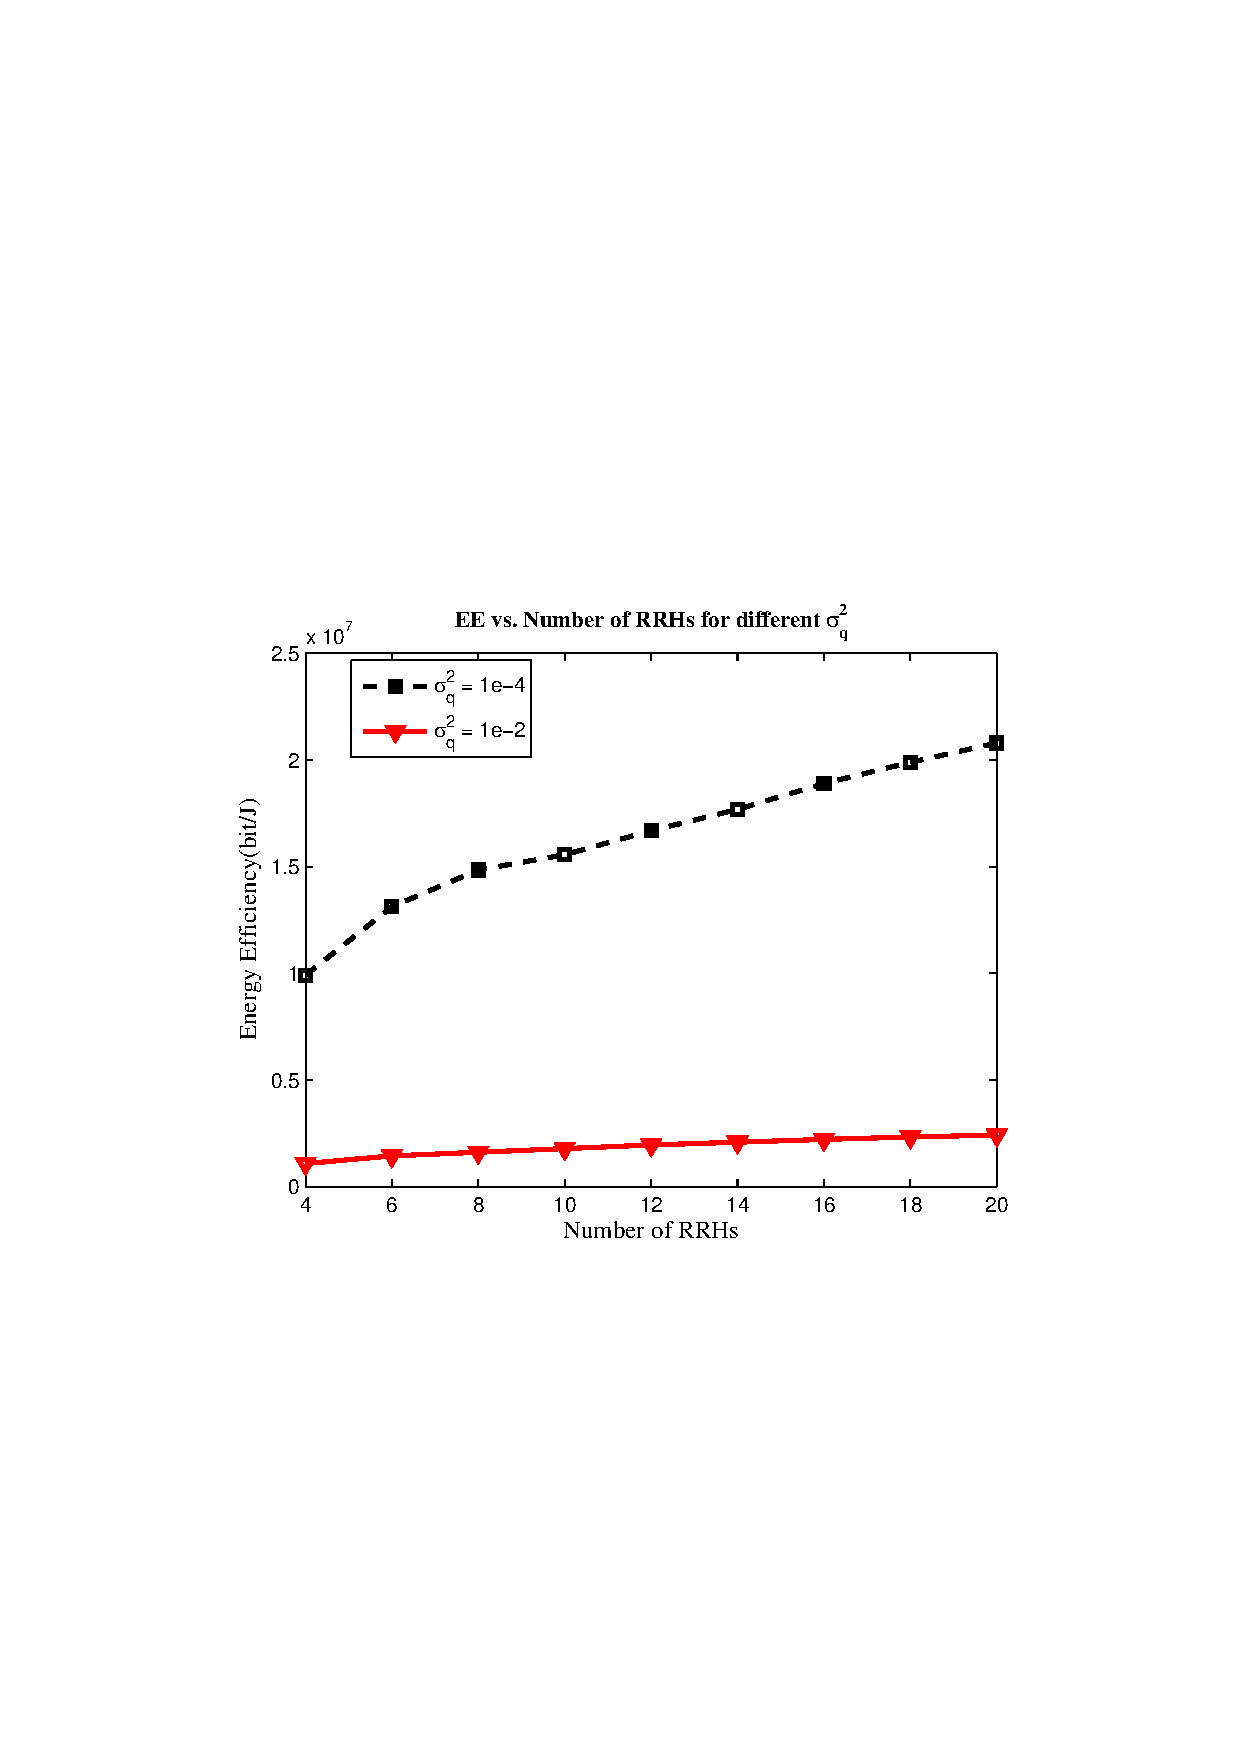
\includegraphics[width=\linewidth]{./fig/varq}
  \caption{ بازدهی انرژی برحسب تعداد واحد های رادیویی تک آنتنه برای واریانس های نویز کوانتیزاسیون متفاوت با فرض وجود 3 کاربر و $P_{max} = 23dBm$}
  \label{fig:varq}
  \end{figure}
 در شکل \ref{fig:varq} ، بازدهی انرژی بر حسب تعداد واحدهای رادیویی تک آنتنه با فرض وجود 3 کاربر و محدودیت 
لینک \lr{fronthaul}، $C_{max} = 5 (bit/s/Hz)$ برای دو نویز کوانتیزاسیون مختلف برای مدل سیستم اول رسم شده است. همانگونه که دیده می شود با افزایش نویز کوانتیزاسیون، بازدهی انرژی برای واحدهای رادیویی مختلف کاهش یافته است و با افزایش واحدهای رادیویی، بازدهی انرژی زیاد می گردد.
\begin{figure}[H]
  \centering
    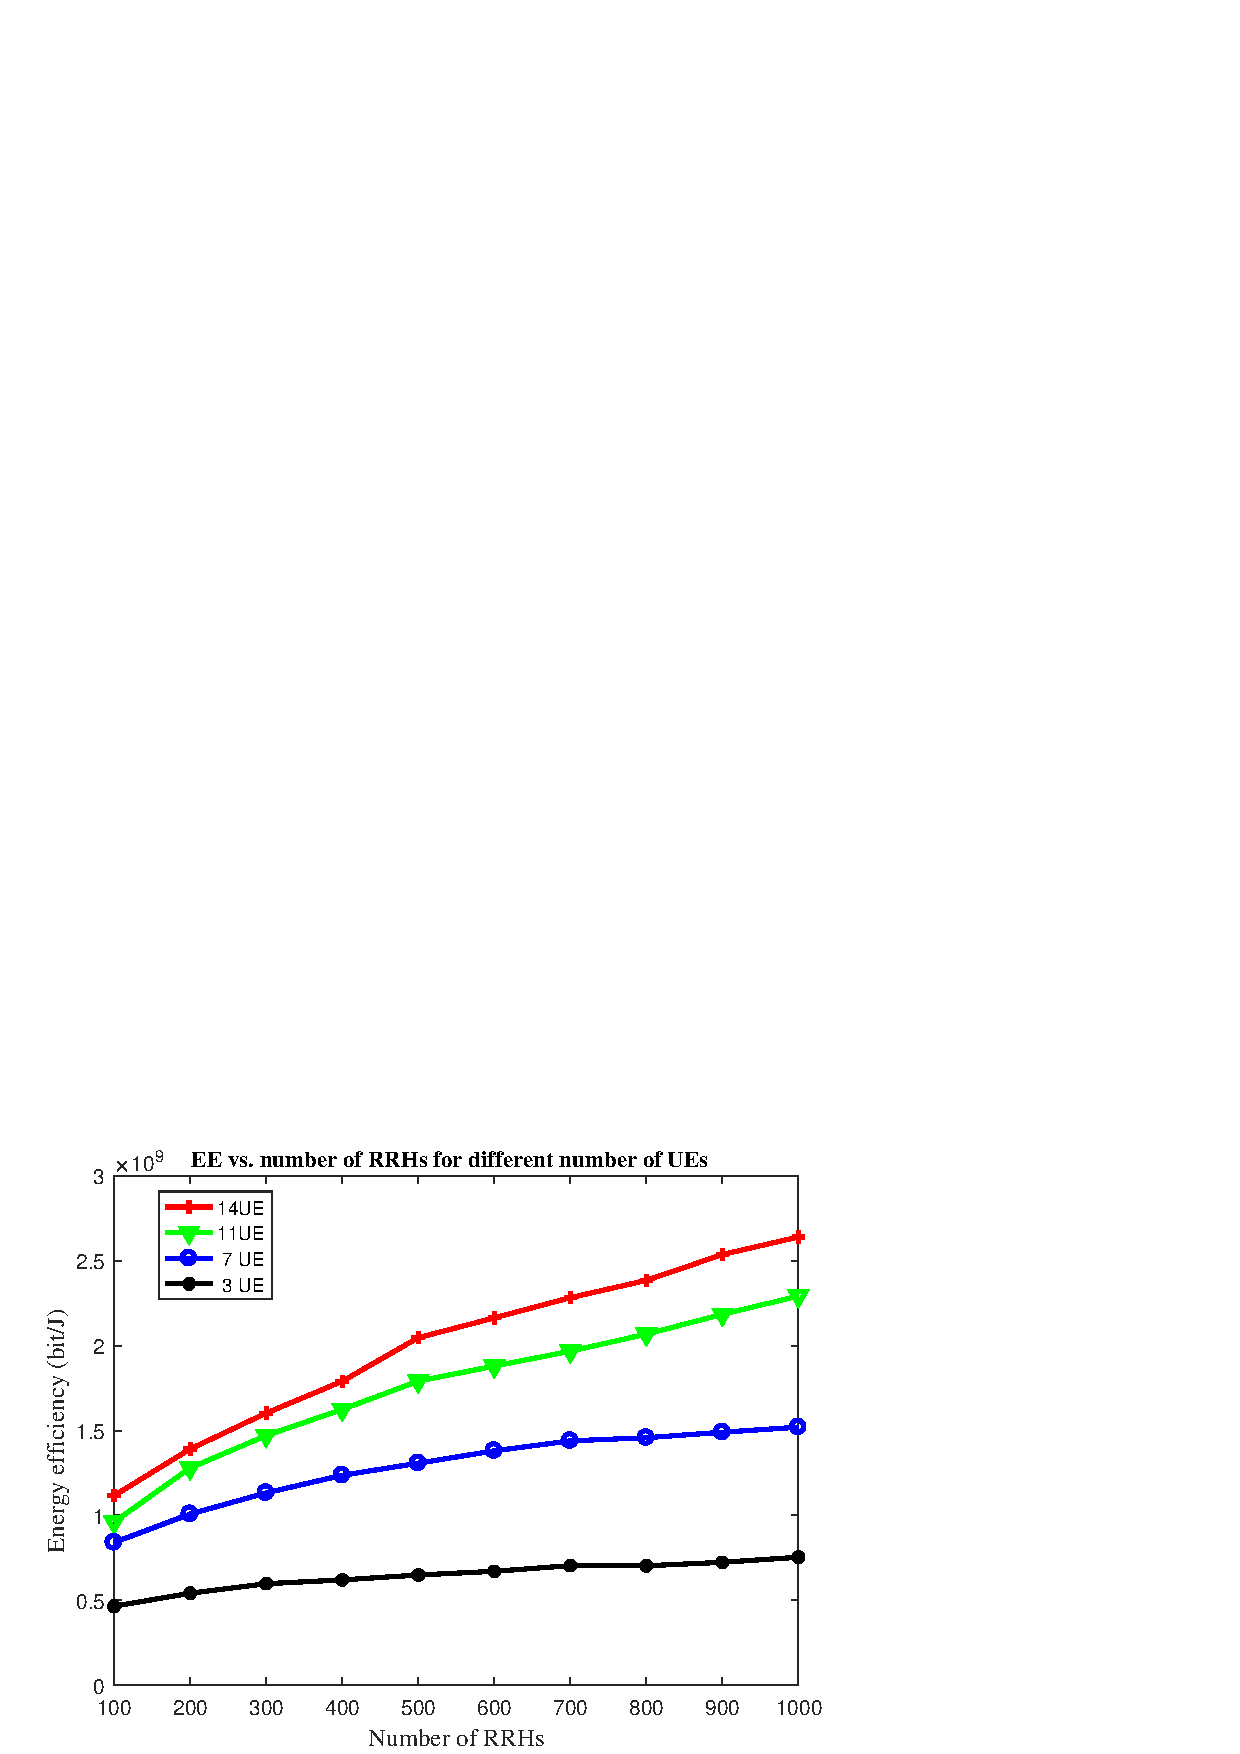
\includegraphics[width=\linewidth]{./fig/eeRRH}
  \caption{ .بازدهی انرژی برحسب تعداد واحدهای رادیویی برای یک خوشه برای تعداد کاربر متفاوت}
  \label{fig:eeRRH2}
  \end{figure}
حال برای مدل سیستم دوم شبیه سازی هایی ارائه می گردد.
%\begin{figure}[H]
%  \centering
%    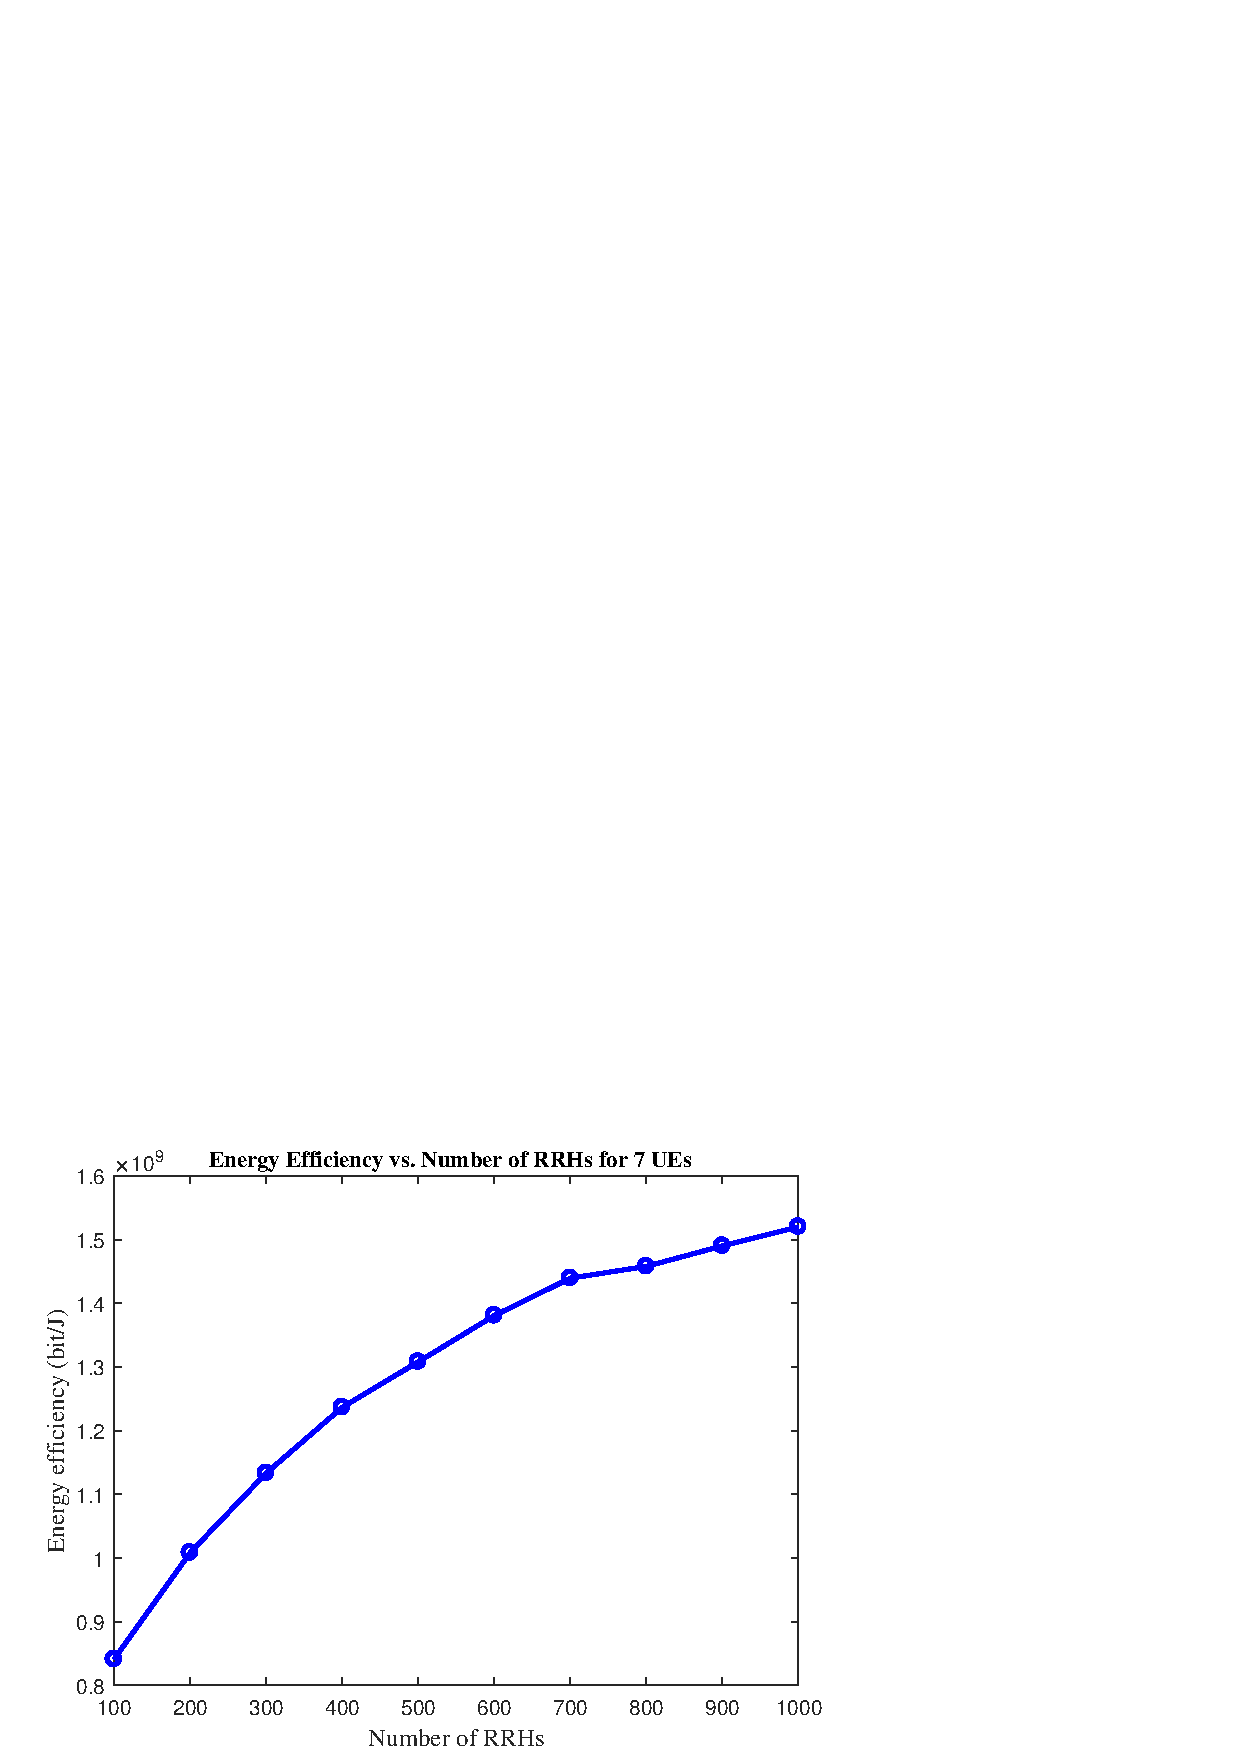
\includegraphics[width=\linewidth]{./fig/UE7}
%  \caption{ٍ بازدهی انرژی برحسب تعداد واحدهای رادیویی برای یک خوشه برای 7 کاربر }
%  \label{fig:UE7}
%  \end{figure}
در مدل سیستم دوم با فرض اینکه در ابتدا خوشه بندی صورت نگرفته باشد، با استفاده از روش الگوریتم تکرار شونده، بازدهی انرژی را برحسب تعداد واحدهای رادیویی برای یک خوشه با تعداد کاربران متفاوت  در شکل \eqref{fig:eeRRH2} با فرض استفاده از پیش کدگذاری \lr{MRT} رسم شده است. در این شکل فرض این است که ظرفیت محدود لینک \lr{fronthaul} و همچنین خوشه بندی در نظر گرفته نشده است. همانطور که در شکل \eqref{fig:eeRRH2} می بینید با افزایش تعداد واحدهای رادیویی، بازدهی انرژی بهبود می یابد. \newline
همچنین برای  شرایط گفته شده، در شکل \eqref{fig:eeUE}، بازدهی انرژی برحسب تعداد کاربران برای دو سری واحدهای رادیویی مختلف کشیده شده است.
\begin{figure}[H]
  \centering
    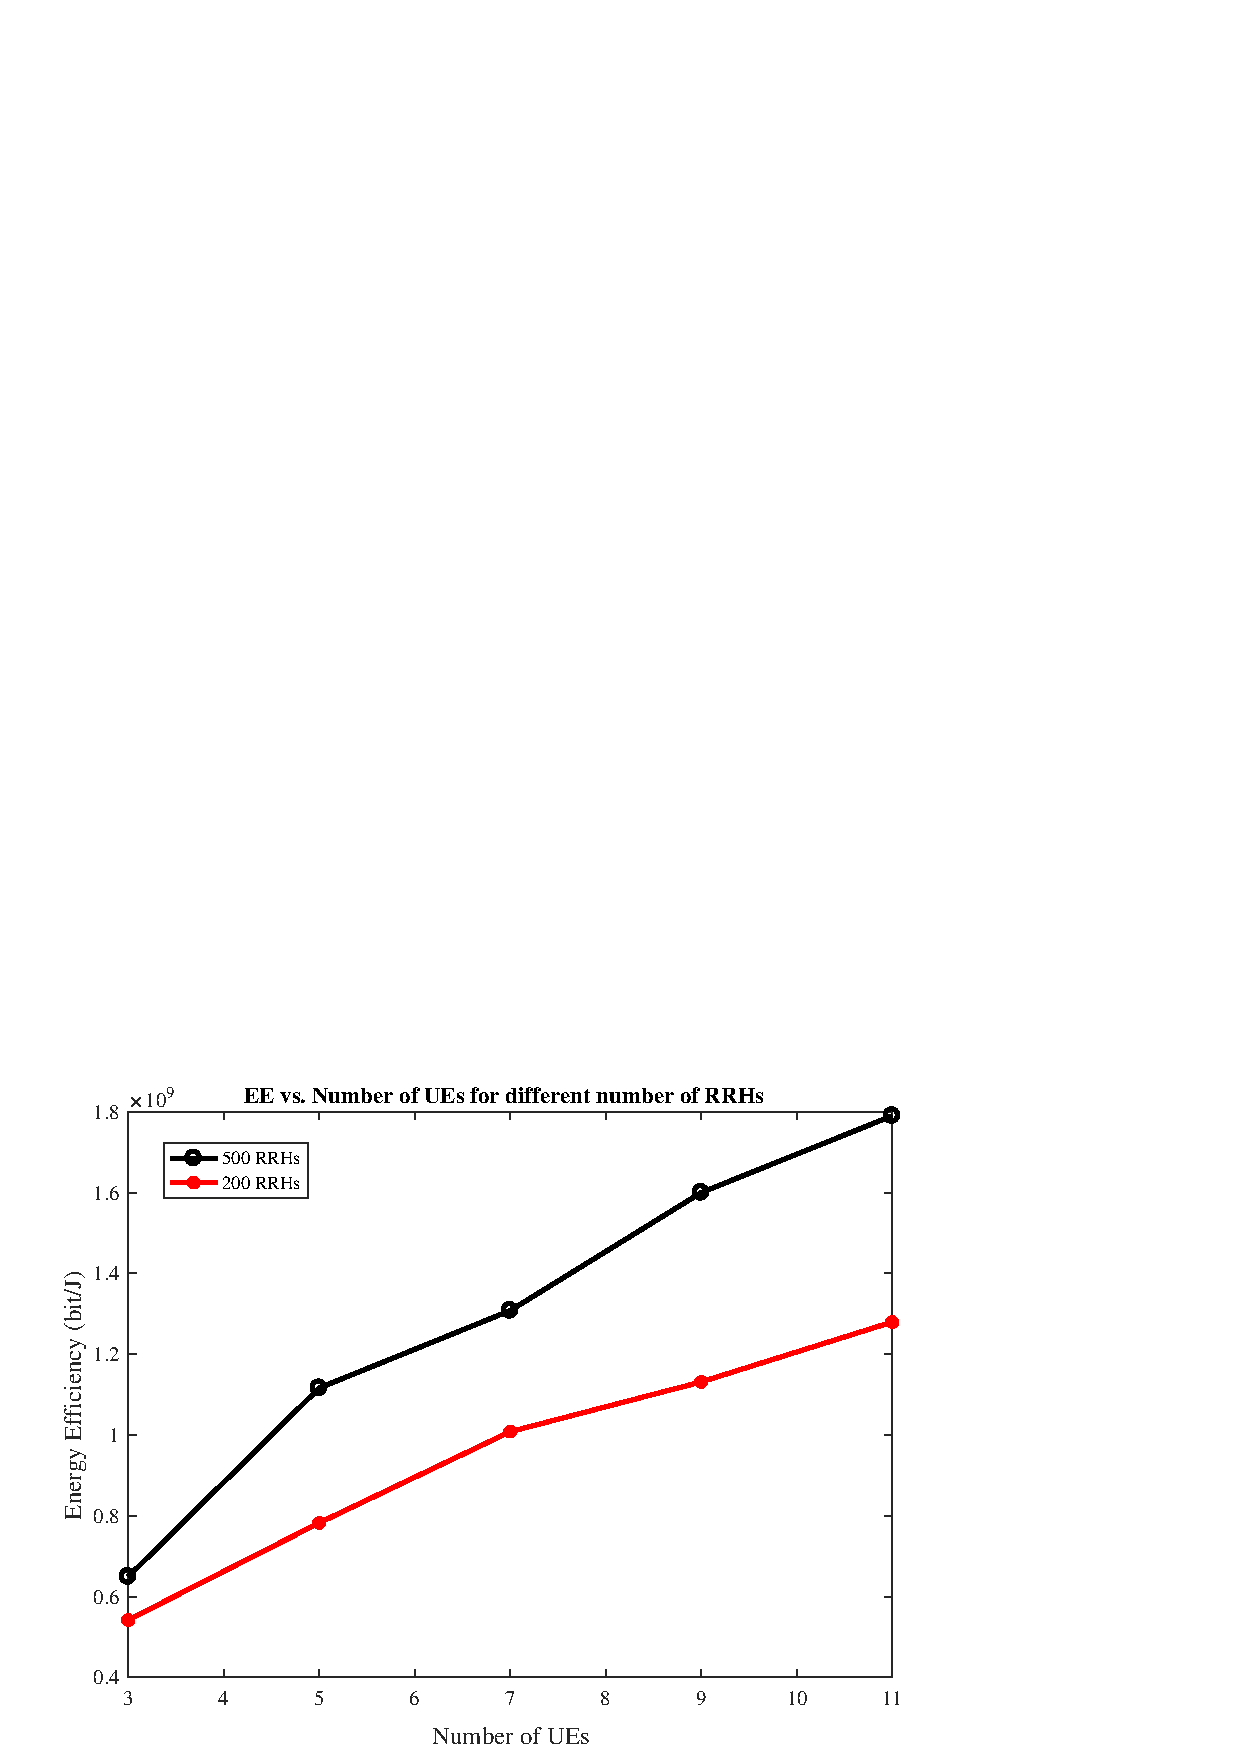
\includegraphics[width=\linewidth]{./fig/eeUE}
  \caption{ٍ بازدهی انرژی برحسب تعداد واحدهای رادیویی برای یک خوشه برای تعداد کاربر متفاوت}
  \label{fig:eeUE}
  \end{figure}
  حال میزان بازدهی انرژی برحسب تعداد واحدهای رادیویی برای دو نوع پیش کدگذاری \lr{MRT} و \lr{MMSE}  برای 3 کاربر در شکل ، نمایش داده شده است.
  با توجه به شکل، پیش کدگذاری \lr{MMSE}، منجر به بازدهی انرژی بیشتری می گردد زیرا با افزایش کاربران تداخل بیشتر شده و پیش کدگذاری \lr{MMSE} در حذف تداخل بهتر از \lr{MRT} عمل می کند.
  
\begin{figure}[H]
  \centering
    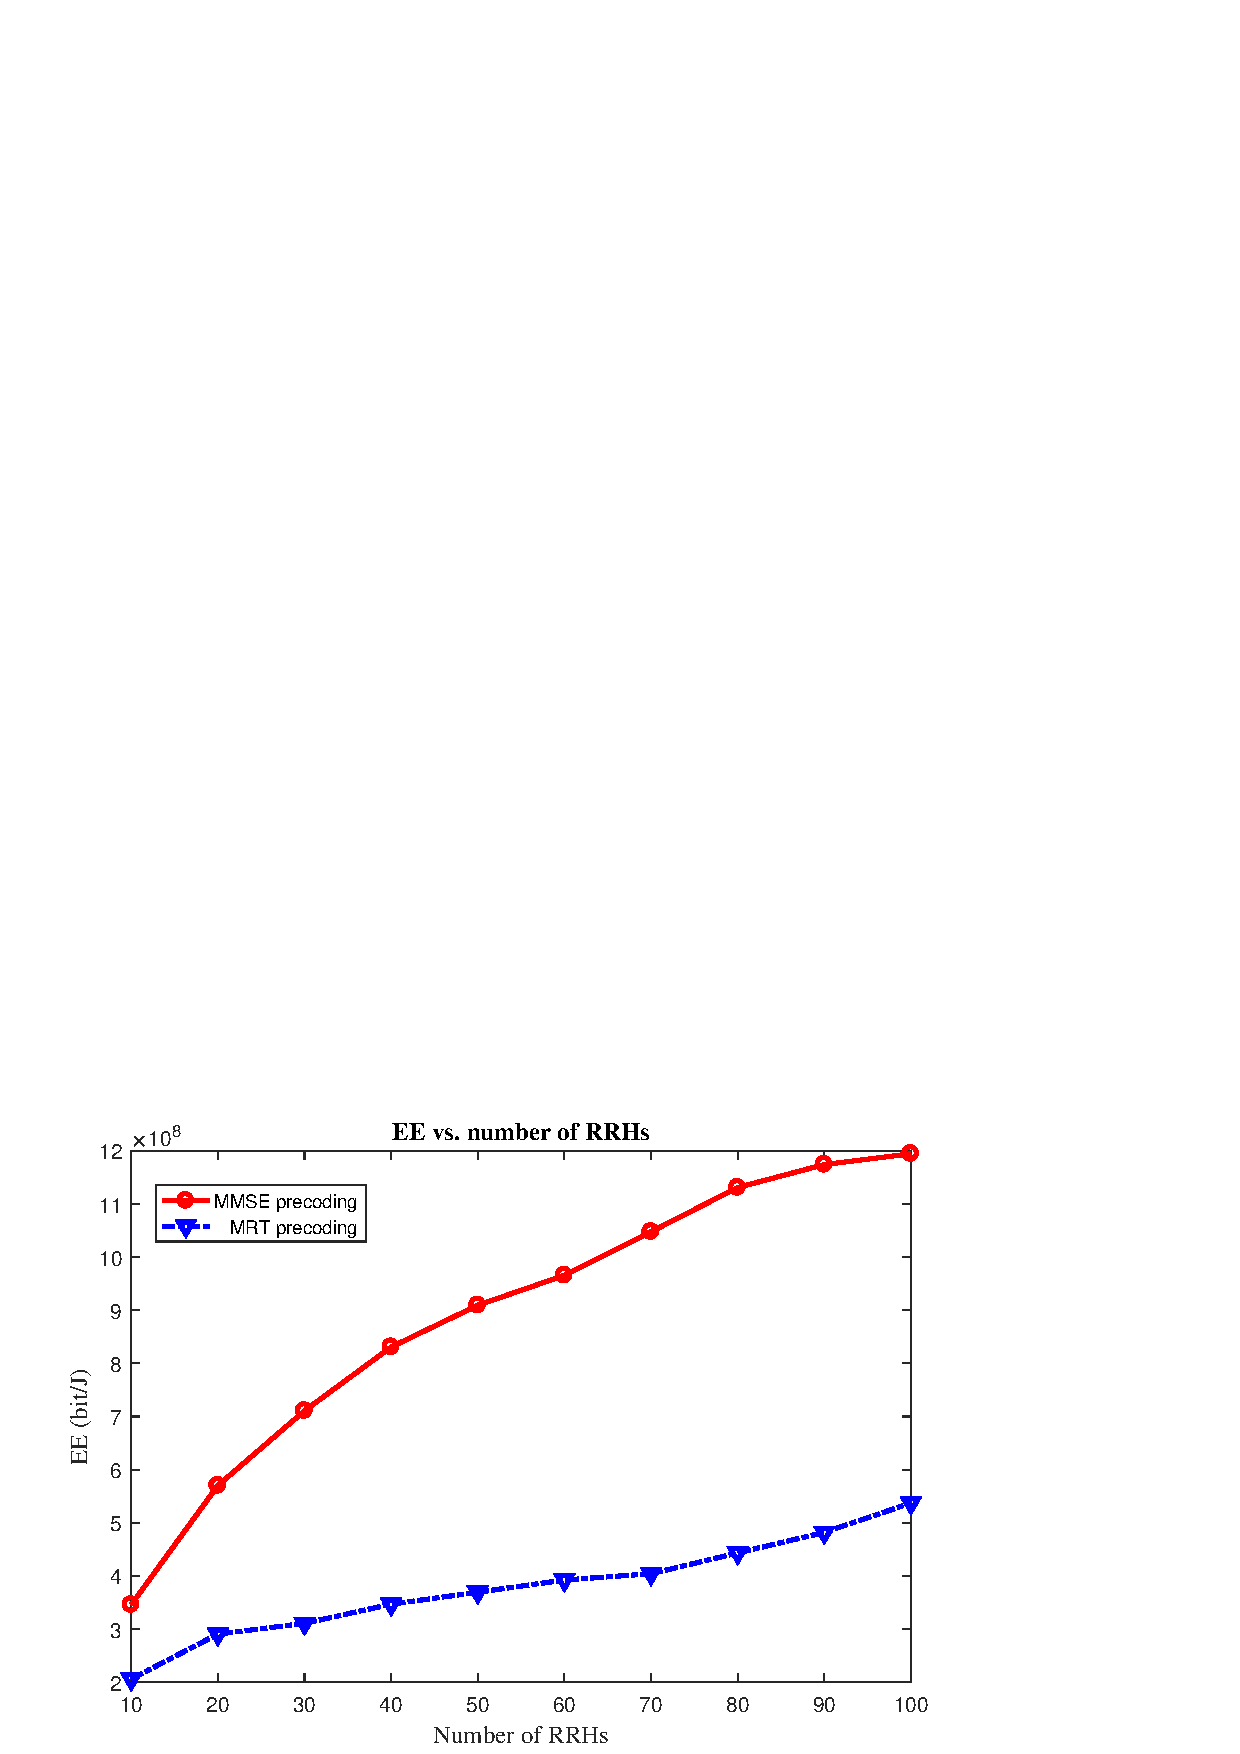
\includegraphics[width=\linewidth]{./fig/precode}
  \caption{
  بازدهی انرژی برحسب تعداد واحدهای رادیویی برای 3 کاربر در دو حالت با پیش کدگذاری متفاوت. }
  \label{fig:precode}
  \end{figure}
  همچنین در شکل \ref{fig:clus}، با فرض وجود 3 خوشه و 3 کاربر در هر خوشه بازدهی انرژی بر حسب تعداد واحدهای رادویی در هر خوشه رسم شده است که در شکل با افزایش تعدا واحدهای رادیویی در هر خوشه بازدهی افزایش می یابد.
  \begin{figure}[H]
  \centering
    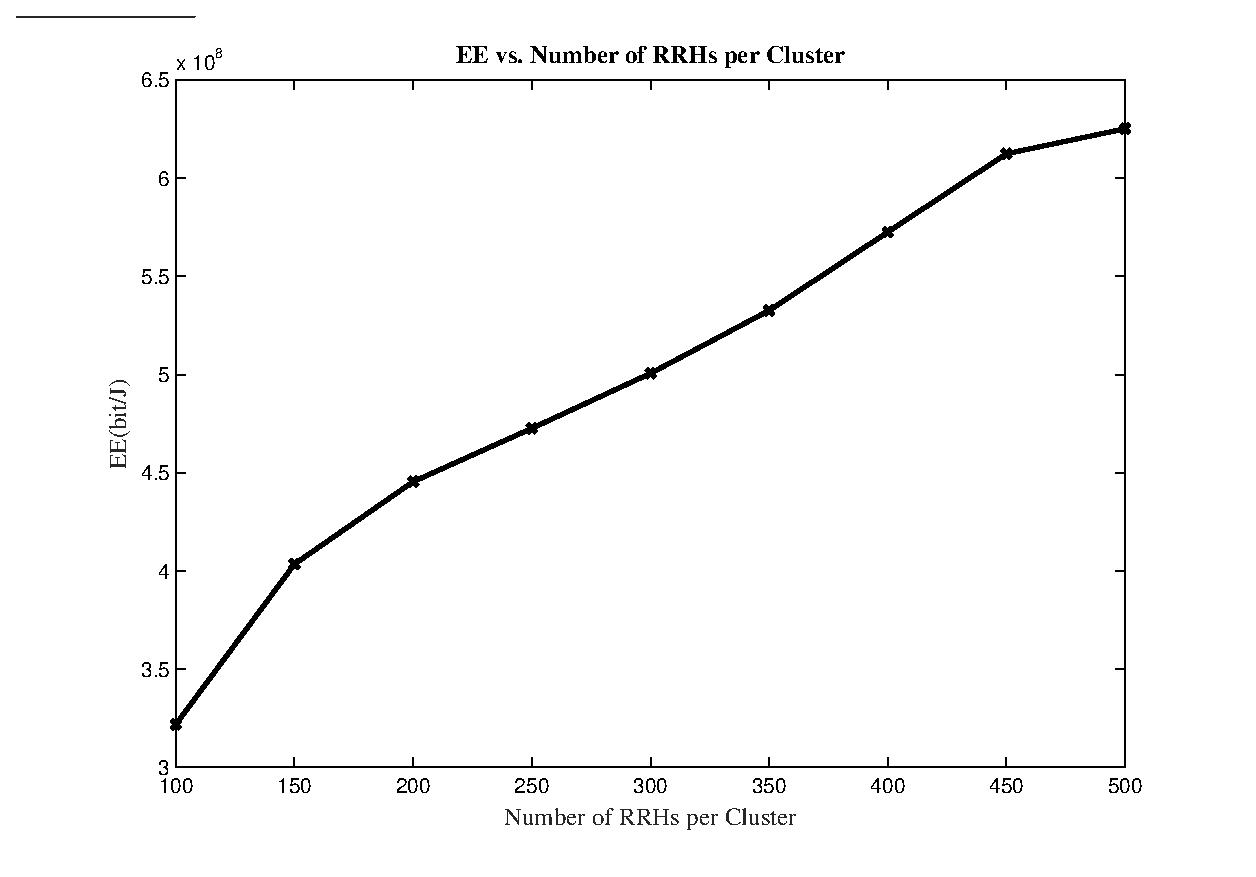
\includegraphics[width=\linewidth]{./fig/f2}
  \caption{
  بازدهی انرژی بر حسب تعداد واحدهای رادیویی با وجود 3 خوشه. }
  \label{fig:clus}
  \end{figure}
\section{لینک فراسو}
در این قسمت کارهای انجام شده در زمینه ی سیستمهای  \lr{MIMO C-RAN}  را در حالت فراسو مورد بررسی قرار گرفته است. در حالت فراسو، پیام از کاربران به واحد رادیویی ارسال می گردد و از طریق لینک \lr{fronthaul} که فیبر نوری است به واحد کنترل برای پردازش انتقال می یابد.
\subsection{مدل سیستم اول}
هدف از این بخش، بررسی لینک فراسو برای مدل سیستم خاص می باشد\cite{ul_dl,ulSimeone, Fronthaul, precodSimeone}. که در شکل \eqref{fig:ul2}، مسیر انتقال پیام از واحد رادیویی به واحد کنترل نمایش داده شده است.
فرض بر این است که در این حالت، سیستم شامل $N_U$ تا کاربر و $N_R$ 
تا واحد رادیویی است. 

\begin{figure}[H]
  \centering
    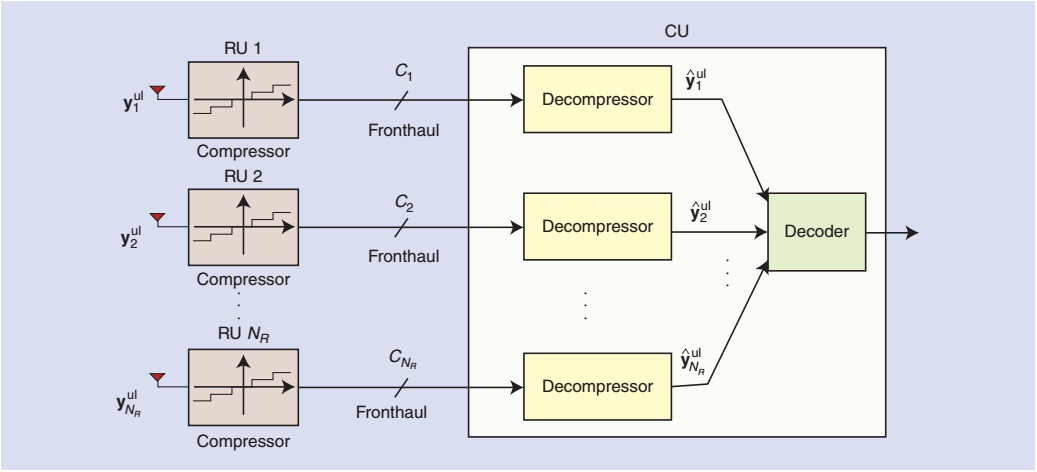
\includegraphics[width=\linewidth, height=6cm]{ul2}
  \caption{مسیر انتقال پیام در لینک فراسو \cite{Fronthaul}.}
  \label{fig:ul2}
\end{figure}
در اینجا همانند لینک فروسو، ساختار سیستم به صورت \lr{MIMO C-RAN} می باشد.  همچنین فرض می کنیم که هر واحد رادیویی دارای $N_r$ تا آنتن و هر کاربر تک آنتنه می باشد.\newline
در این مدل سیستم  زمان ارسال پیام به دو بخش تقسیم می گردد. بخشی از زمان در ابتدا برای ارسال پایلوت و بخشی دیگر صرف ارسال پیام می گردد. کل زمان ارسال پیام را $T$ در نظر گرفته  که به دو بخش $T_p$ برای ارسال پایلوت و یادگیری کانال و $T_d$ برای ارسال داده می باشد:
\begin{equation}
T = T_p + T_d
\end{equation}
سیگنال ارسالی توسط هر کاربر دارای ابعاد $1 \times T$ می باشد.
سیگنال ارسالی توسط کاربر $i$ام با نماد $\boldsymbol{X}_i$نشان داده شده که دارای توان 
 $\frac{1}{T} \mathit{E}[||\boldsymbol{X}_{i} ||^2] = P_{i}$
است. این سیگنال
به دو قسمت تقسیم می شود. قسمت اول
 $X_{p,i}$
  برای ارسال پایلوت است و دارای توان 
 $\frac{1}{T_p} \mathit{E}[||\boldsymbol{X}_{p,i} ||^2] = P_{p,i}$
می باشد و قسمت دوم
 $X_{d,i}$
 برای ارسال داده است و دارای توان 
 $\frac{1}{T_d} \mathit{E}[||\boldsymbol{X}_{d,i} ||^2] = P_{d,i}$
 می باشد.
 همچنین این توانها در معادله ی داده شده صدق می کنند:
 \begin{equation}
 \frac{T_p}{T}P_{p,i} +  \frac{T_d}{T}P_{d,i} = P_i
 \end{equation}
به علاوه سیگنال  یادگیری کانال که همان پایلوت است به صورت
 $\boldsymbol{X}_p = [\boldsymbol{X}_{p,1}^T,...,\boldsymbol{X}_{p,N_U}^T]^T$
است و
  $\boldsymbol{X}_d = [\boldsymbol{X}_{d,1}^T,...,\boldsymbol{X}_{d,N_U}^T]^T$
  سیگنال داده است.
 علاوه بر این،  
 $\boldsymbol{X}_p = \sqrt{P_p} \boldsymbol{S}_p$
 و 
  $\boldsymbol{X}_d = \sqrt{P_d} \boldsymbol{S}_d$
  که در اینجا $\boldsymbol{S}_p$ و $\boldsymbol{S}_d$ به ترتیب بردارهای $N_U \times T$ هستند 
  که نرمالیزه شده اند.
  
  
  پیام دریافتی توسط  $j$ امین واحد رادیویی برای دو حالت پیام یادگیری کانال و داده در ادامه بیان شده است:
  \begin{equation}\label{ypd}
  \begin{split}
 \boldsymbol{Y}_{p,j} &= \sqrt{P_p} \boldsymbol{H}_j \boldsymbol{S}_p + \boldsymbol{Z}_{p,j}\\
  \boldsymbol{Y}_{d,j} &= \sqrt{P_d} \boldsymbol{H}_j \boldsymbol{S}_d + \boldsymbol{Z}_{d,j}\\
 \end{split}
  \end{equation}
  در معادله ی \eqref{ypd}، $\boldsymbol{Z}_{p,j}$ و $\boldsymbol{Z}_{d,j}$ نویز گوسی جمع شونده
   $\boldsymbol{Z} \backsim \mathcal{N}(0,1)$ 
   می باشند و بردارهای آنها به ترتیب دارای $N_r \times T_p$ و
   $ N_r \times T_d$
     ابعاد است. همچنین بردار$\boldsymbol{H}_j $ ،نشان دهنده ی بردار کانال از کاربران به  $j$ امین واحد رادیویی می باشد که می توان به صورت $\boldsymbol{H}_j = [\boldsymbol{h}_{j,1},..., \boldsymbol{h}_{j,N_U}]$ بسط داد و دارای ابعاد  $N_r \times N_u$ می باشد.
    بردار کانال  
    $\boldsymbol{h}_{j,1}$
     در اینجا به صورت 
     $iid \backsim \mathcal{N}(0,\alpha_{j,i})$
       مدل شده است که 
      $\alpha_{j,i} = \frac{1}{1 + \frac{d_{ji}}{d_0}}$
      می باشد.
      
      حال، همانطور که در شکل \eqref{fig:ul2} ، دیده می شود، پیام دریافتی توسط واحد رادیویی، فشرده سازی می گردد \cite{uljmimo} که در اینجا برای دو بخش پایلوت و داده جداگانه بررسی می کنیم.
      \subsubsection{ مرحله ی یادگیری کانال   }
    در طول این مرحله، فشرده سازی و کوانتیزاسیون برای سیگنال   
    $ \boldsymbol{Y}_{p}$
    اعمال می گردد و می توان به حالت زیر نوشت
    
      \begin{equation}\label{yp}
      \hat{\boldsymbol{Y}}_{p} = \boldsymbol{Y}_{p} + \boldsymbol{Q}_{p}
      \end{equation}
      در معادله ی \eqref{yp}، 
       $\boldsymbol{Q}_{p} \backsim \mathcal{N}(0,\sigma_{p}^2 \boldsymbol{I} )$ 
         و \lr{iid}
       
         می باشد که
      $\sigma_{p}^2$
      تابع محدودیت لینک   
      \lr{fronthaul}
      می باشد.
       \newline
       حال با توجه به معادله ی  \eqref{yp}
       کانال بین کاربران و واحدهای رادیویی بوسیله ی \lr{MMSE} با خطا تخمین زده می شوند.
       \begin{equation}
       \boldsymbol{H} = \hat{\boldsymbol{H}} + \boldsymbol{E}
       \end{equation}
       که کانال تخمین زده ی $\hat{\boldsymbol{H}}$، ماتریس گوسی به صورت
        $\hat{\boldsymbol{H}} :iid \backsim \mathcal{N}(0,\sigma_{\hat{h}}^2)$ 
         و  $\hat{\boldsymbol{E}}: iid \backsim \mathcal{N}(0,\sigma_{e}^2)$  می باشد.
        همچنین $\sigma_{\hat{h}}^2 =\alpha - \sigma_{e}^2$ است.
      
     
  \subsubsection{ مرحله ی بررسی داده  }
  در این مرحله، داده فشرده سازی و کوانتیزاسیون می گردد.
  
    \begin{equation}\label{yd}
      \hat{\boldsymbol{Y}}_{d} = \boldsymbol{Y}_{d} + \boldsymbol{Q}_{d}
      \end{equation}
      در معادله ی \eqref{yd}،  $\boldsymbol{Q}_{d} :iid \backsim \mathcal{N}(0,\sigma_{d}^2)$  می باشد.
علاوه بر این نویز معادل به صورت  $\boldsymbol{N}_{d}=\boldsymbol{E} \boldsymbol{X}_{d}+\boldsymbol{Z}_{d}+\boldsymbol{Q}_{d}$ تعریف می گردد.  
      همچنین داریم:
      
      
  \begin{equation}
  \hat{\boldsymbol{Y}}_{d} =  \hat{\boldsymbol{H}} \boldsymbol{X}_{d} + \boldsymbol{N}_{d}
  \end{equation}
  که در اینجا
    $\boldsymbol{N}_{d} :iid$
    با میانگین صفر و توان 
  $  1+\sigma_{d}^2 + P_d \sigma_{e}^2$
  است که نویز گوسی می باشد که مستقل از 
  $\boldsymbol{X}_{d} $
  نیست.
 \subsubsection{صورت مسئله}
 در ابتدای این بخش نرخ قابل دسترس و ظرفیت لینک محاسبه می گردد سپس  صورت مسئله بیان می شود.
 کران پایین برای نرخ قابل دسترس برای مدل سیستم بیان شده با توجه به مقالات به صورت زیر است:
 \begin{equation}
 R = \frac{T_d}{T} \mathcal{E}\{\log_2{det (\boldsymbol{I}_{N_r}+\rho_{eff} \hat{\boldsymbol{H}} \hat{\boldsymbol{H}}^{H} )}\}
 \end{equation}
 که در اینجا $\rho_{eff} = P_d / ( 1+\sigma_{d}^2 + P_d \sigma_{e}^2)$ می باشد.
 علاوه بر این در ادامه ظرفیت لینک \lr{frotnhaul} را بدست می آید. در اینجا فرض بر این است که  $C_p$ ظرفیت بخش پایلوت و $       C_d$   ظرفیت داده در این لینک باشد در نتیجه ظرفیت کل لینک برابر است با 
 $\bar{C} = C_p +C_d.$
که در اینجا
 \begin{equation}
 \begin{split}
 C_p & = \frac{Tp N_r}{T} \log_2 (1 + \frac{P_p \alpha +1}{\sigma_p^2})\\
  C_d & = \frac{Td N_r}{T} \log_2 (1 + \frac{P_d \alpha +1}{\sigma_d^2})
 \end{split}
 \end{equation}
 است.
 حال در این حالت، مجموع نرخ های قابل دسترس براساس محدودیت ظرفیت لینک \lr{fronthaul} و محدودیت توان هر واحد رادیویی، بیشینه می گردد:
\begin{equation}
\begin{aligned}
\max\limits_{P_d,P_p}   \quad &   \sum R(P_d)\\
\text{\lr{subject to}} \quad  & \bar{P}_i \leq P_{max} \ \  \forall i \\
&\bar{C} ({P_d,P_p})\leq C^{th} \\
\end{aligned}
\end{equation}
 \subsection{مدل سیستم دوم}
 در این قسمت مدل سیستم دیگری برای لینک فراسو در نظر گرفته شده است \cite{ofdma,ulCompression,dlulP}.
 در این مدل سیستم فرض بر این است که 
 $N$
 تا واحد رادیویی داریم که $K$ کاربر را سرویس دهی می کنند همچنین فرض بر این است که واحدهای رادیویی و کاربران تک آنتنه هستند. برخلاف مدل سیستم قبل، در این بخش یادگیری کانال و یا پایلوت در مدل سیستم بیان نمی شود و صرفا مرحله ی پردازش داده مورد بررسی قرار می گیرد. همچنین از خوشه بندی کاربران و واحدهای رادیویی صرف نظر می گردد.
 سیگنال دریافتی توسط $n$ امین واحد رادیویی که با $y_n$  نمایش می دهیم به وسیله ی معادله ی زیر بدست می آید:
 \begin{equation}
 y_n = \sum_{k=1}^{K} h_{n,k} \sqrt{p_k} s_k + z_n
 \end{equation}
 که در اینجا، $h_{n,k}$ مقدار کانال از $k$ امین کاربر به $n$ امین واحد رادیویی می باشد. علاوه بر این، $p_k$ توان ارسالی کاربر $k$ ام می باشد و $s_k$ پیام کاربر $k$ ام است. نیز $z_n$ نویز گوسی جمع شونده ی دریافتی برای $n$ امین واحد رادیویی است که دارای میانگین صفر و واریانس $\sigma_n^2$ می باشد.
 $z_n \backsim \mathcal{N}(0,\sigma_n^2)$ 

همچنین همانطور که قبلا گفته شده به دلیل محدودیت ظرفیت لینک \lr{fronthaul} پیام دریافتی توسط واحد رادیویی فشرده شده و سپس از طریق این لینک به واحد کنترل ارسال می گردد.
پیام فشرده شده به این صورت بیان می گردد.
\begin{equation}\label{yq}
\tilde{y}_n = y_n + q_n
\end{equation} 
که در اینجا
 $q_n \backsim \mathcal{N}(0,\sigma_q^2) \ \ \forall n$ 
 نویز گوسی جمع شونده می باشد.
 در نتیجه با توجه به رابطه ی \eqref{yq}، نرخ انتقال پیام از $n$ امین واحد رادیویی به واحد کنترل از طریق لینک \lr{fronthaul} به شرح زیر است.
 \begin{equation}
 C_n = B \log_2 (1+ \frac{\sum_{k=1}^{K} |h_{n,k}|^2 p_k}{\sigma_q^2})
 \end{equation}
 
پیام فشرده شده پس از انتقال به واحد کنترل از طریق لینک با ظرفیت محدود، در این واحد کنترل به صورت خطی ترکیب می گردد تا بتوان سیگنال هر پیام را تخمین زد.
در نتیجه برای بدست آوردن سیگنال $s_k$ که توسط کاربر ارسال شده است از روش تشخیص \lr{MRC} که همان ترکیب خطی بین پیامهای دریافتی است، استفاده می نماییم.
\begin{equation}\label{sk}
\hat{s}_k = \boldsymbol{w}_k^H \tilde{\boldsymbol{y}}
\end{equation}
در معادله ی بالا،
 $\boldsymbol{w}_k = [w_{1,k},...,w{N,k}]$
 
 همان بردار تشخیص است که $w_{i,k} = h_{i,k}^*$ می باشد.
همچنین در اینجا بردار $\tilde{\boldsymbol{y}}$ به حالت مقابل تعریف می شود، 
$\tilde{\boldsymbol{y}} = [ \tilde{y}_1,..., \tilde{y}_N]$
حال می توان معادله ی \eqref{sk} را به شکل زیر بسط داد.
\begin{equation}\label{skext}
\begin{split}
\hat{s}_k &= \underbrace{\boldsymbol{w}_k^H \boldsymbol{h}_k \sqrt{P}_k s_k }_{\text{(\lr{desired signal})}} \\
&+\underbrace{ \sum_{k=1,j \neq k}^{K}  \boldsymbol{w}_k^H \boldsymbol{h}_j \sqrt{P}_j s_j}_{\text{(\lr{interference signal})}}  \\
&+ \underbrace{\boldsymbol{w}_k^H (\boldsymbol{z}+\boldsymbol{q})}_{\text{(\lr{quantisation and additive noise})}}\\
\end{split}
\end{equation}
در معادله ی ذکر شده، $\boldsymbol{h}_k$ بردار کانال از کاربر $k$ ام به تمام واحدهای رادیویی است که می توان به صورت $\boldsymbol{h}_k = [h_{1,k},...,h_{N,k}]$ نوشت. به همین منوال،
 $\boldsymbol{z} = [z_{1},...,z_{N}]$
و نیز $
\boldsymbol{q} = [q_{1},...,q_{N}]$
می باشد.
\subsubsection{صورت مسئله}
همان طور که می دانیم نرخ قابل دسترس برای $k$ امین کاربر به این صورت بدست می آید.
\begin{equation}
R_k = B \log_2(1+ \gamma_k)
\end{equation}
که $ \gamma_k$ همان \lr{SINR} برای $k$ امین کاربر می باشد. با توجه به معادله ی \eqref{skext}، $\gamma_k$ از رابطه ی زیر بدست می آید
\begin{equation}
\gamma_k = \frac{p_k |\boldsymbol{w}_k^H \boldsymbol{h}_k|^2}{\sum_{k=1,j \neq k}^{K} p_j |\boldsymbol{w}_k^H \boldsymbol{h}_j|^2 + (\sigma_n^2+\sigma_q^2) ||\boldsymbol{w}_k||^2}
\end{equation}


 همانطور که گفته شد نسبت مجموع نرخ ها در سیستم به کل توان ارسالی کاربرها نشان دهنده ی بازدهی انرژی است که با $\eta$ نمایش داده می شود و می توان اینگونه بیان کرد
\begin{equation}\label{eta1}
\eta(\boldsymbol{P}) = \frac{\sum\limits_{k=1}^{K}{R}_{k} }{ \sum\limits_{k=1}^{K}{p}_{k}}= \frac{R_{total}(\boldsymbol{P})}{P_{UE}(\boldsymbol{P})},
\end{equation}
حال در این مسئله، هدف بیشینه سازی بازدهی انرژی با شروط زیر می باشد:
 \begin{equation}\label{p11}
\begin{aligned}
\max\limits_{\boldsymbol{P}}   \quad &   \eta(\boldsymbol{P})\\
\text{\lr{subject to}} \quad  &  0 \leq {p}_{k} \leq P_{max} && \qquad \forall k,   \\
&{R}_{k} \geq {R}_{k}^{th} && \qquad \forall k, \\ 
&C_{n} \leq C_{n}^{th}  &&\qquad  \forall i, \\
\end{aligned}			
\end{equation}
برای بدست آوردن توان بهینه، از تابع لاگرانژ و الگوریتم تکرار شونده استفاده می شود که در فصل 3 به طور کامل شرح داده می شود.
  \subsection{نتایج عددی}
  در این بخش، نتایج عددی الگوریتم مورد استفاده را برای سیستم  با پرتو دهی \lr{MRT} و با پارامترهای بیان شده در جدول \ref{tab:title3} \cite{ofdma} بیان می شود.
\begin{latin} 
 \begin{table}[H]
 \caption {\rl{پارامترهای شبیه سازی}} \label{tab:title3} 
 \begin{center}
  \begin{tabular}{||c c ||} 
  \hline
  Parameter & Value \\ [0.5ex] 
  \hline\hline
  Number of cluster S & 1 \\ 
  \hline
    The radius of the cell & 500m \\ 
  \hline
  Noise power density & -174dBm/Hz\\
  \hline
  Bandwidth & 1MHz \\
  \hline
 Maxmimun transmit Power & 23dBm \\
  \hline
Circuit Power of whole RRHs & 10dBm \\
  \hline
  Minimum data rate &  0.1bits/sec/Hz \\ [1ex] 
  \hline
 \end{tabular}
 \end{center}
 \end{table}
 \end{latin}

\begin{figure}[H]
  \centering
    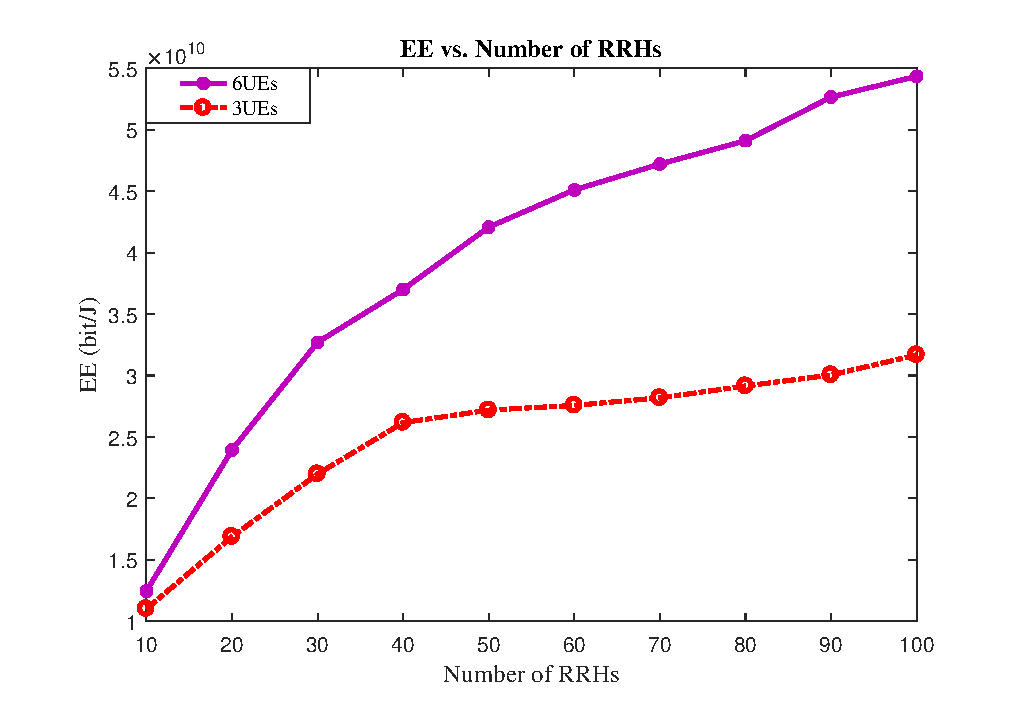
\includegraphics[width=\linewidth]{./fig/rrhul}
  \caption{ٍ بازدهی انرژی برحسب تعداد واحدهای رادیویی برای یک خوشه برای 2 کاربر متفاوت}
  \label{fig:rrhul}
  \end{figure}
 حال بازدهی انرژی را برحسب تعداد واحدهای رادیویی برای یک خوشه با تعداد کاربران متفاوت  در شکل \eqref{fig:eeRRH2} با فرض استفاده از پیش کدگذاری \lr{MRT} رسم شده است. در این شکل فرض این است که ظرفیت محدود لینک \lr{fronthaul} و همچنین خوشه بندی در نظر گرفته نشده است. همانطور که در شکل می بینید با افزایش تعداد واحدهای رادیویی، بازدهی انرژی بهبود می یابد.

\begin{figure}[H]
  \centering
    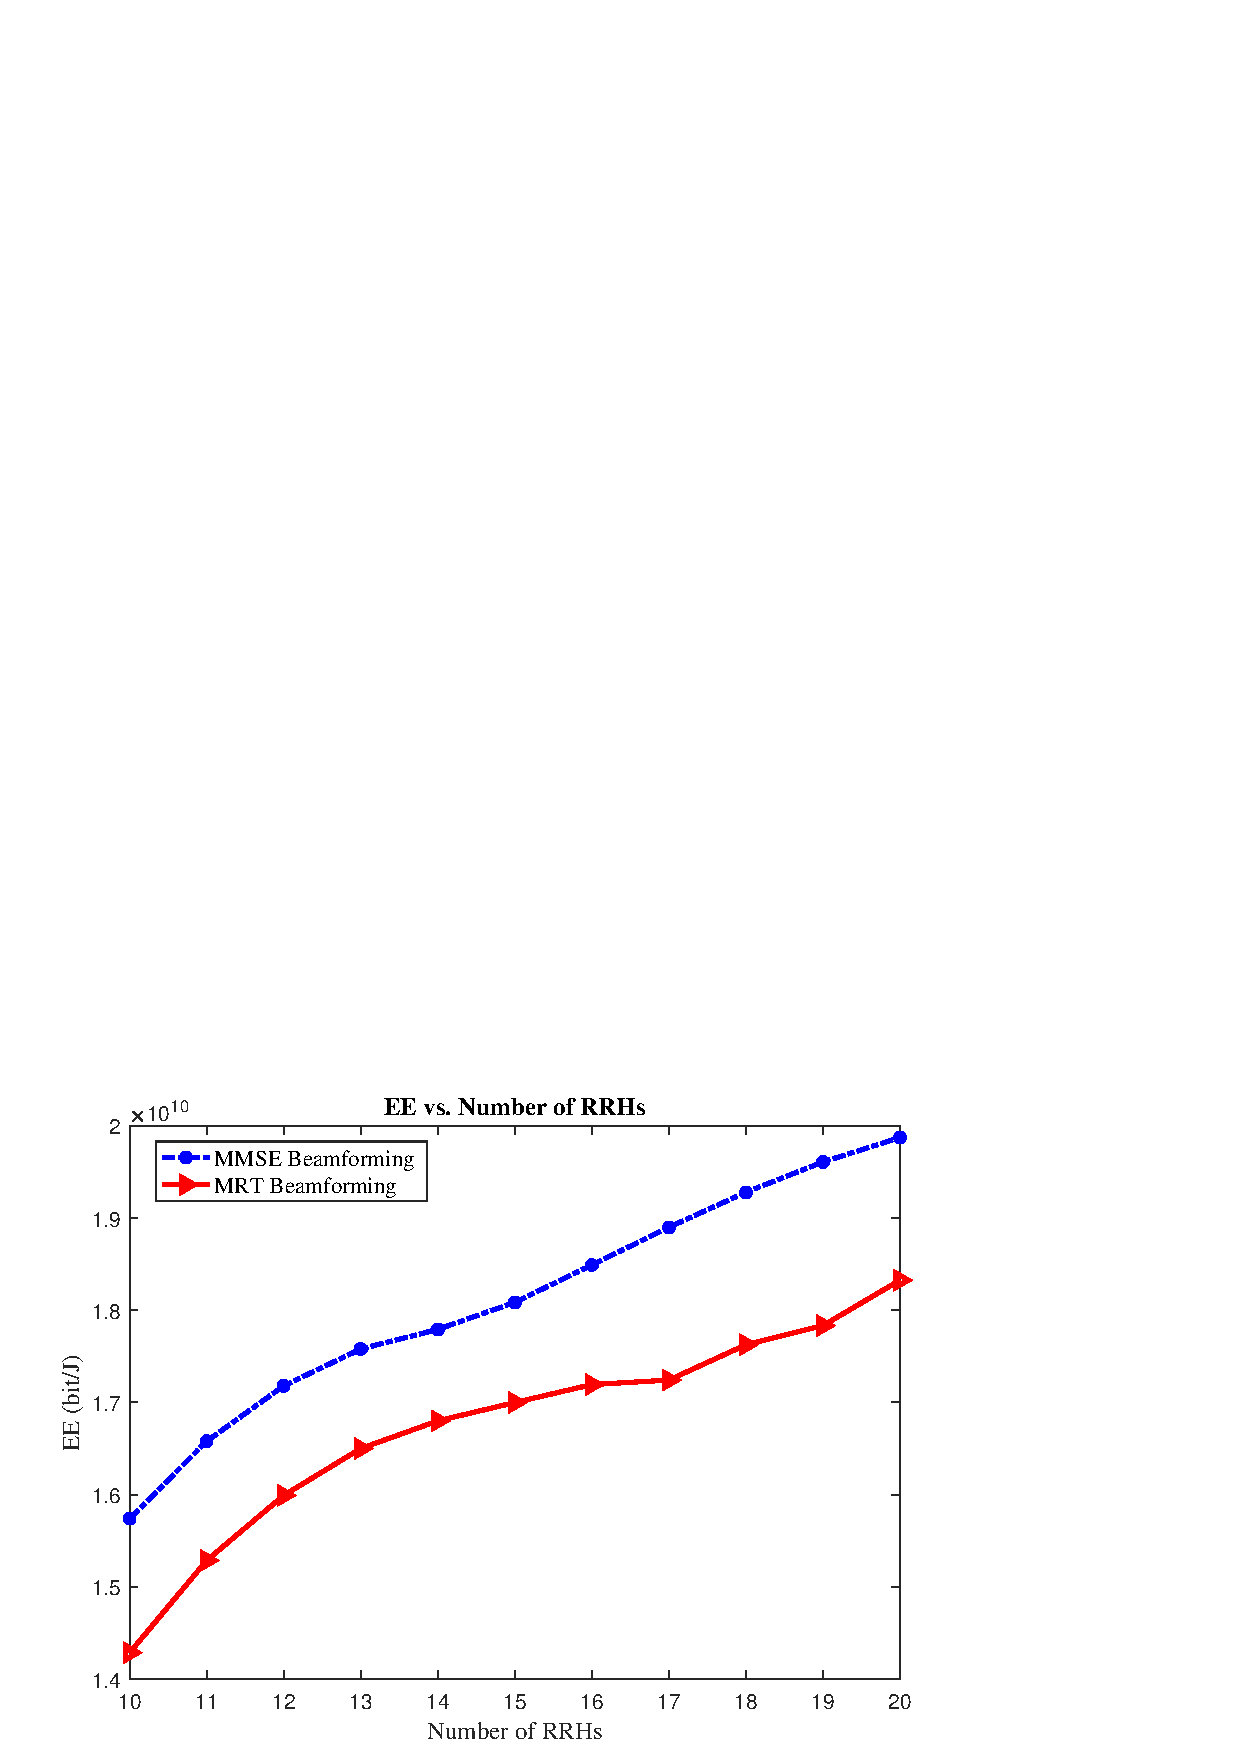
\includegraphics[width=\linewidth]{./fig/beamforming}
  \caption{ٍ بازدهی انرژی برحسب تعداد واحدهای رادیویی برای2 کاربر  در دو حالت با پرتودهی متفاوت }
  \label{fig:beam}
  \end{figure}
      حال میزان بازدهی انرژی برحسب تعداد واحدهای رادیویی برای دو نوع پیش کدگذاری \lr{MRT} و \lr{MMSE}  برای 2 کاربربا فرض های گفته شده برای شکل قبلی،  در شکل \ref{fig:beam} ، رسم کرده ایم.
  با توجه به شکل ، می توان فهمید که پیش کدگذاری \lr{MMSE}، منجر به بازدهی انرژی بیشتری می گردد زیرا \lr{MRT} اثر بیشتری در حذف نویز داشته در صورتی که \lr{MMSE} تداخل را بهتر از بین می برد و در اینجا تاثیر نویز از تداخل کمتر است .


 \begin{figure}[H]
  \centering
    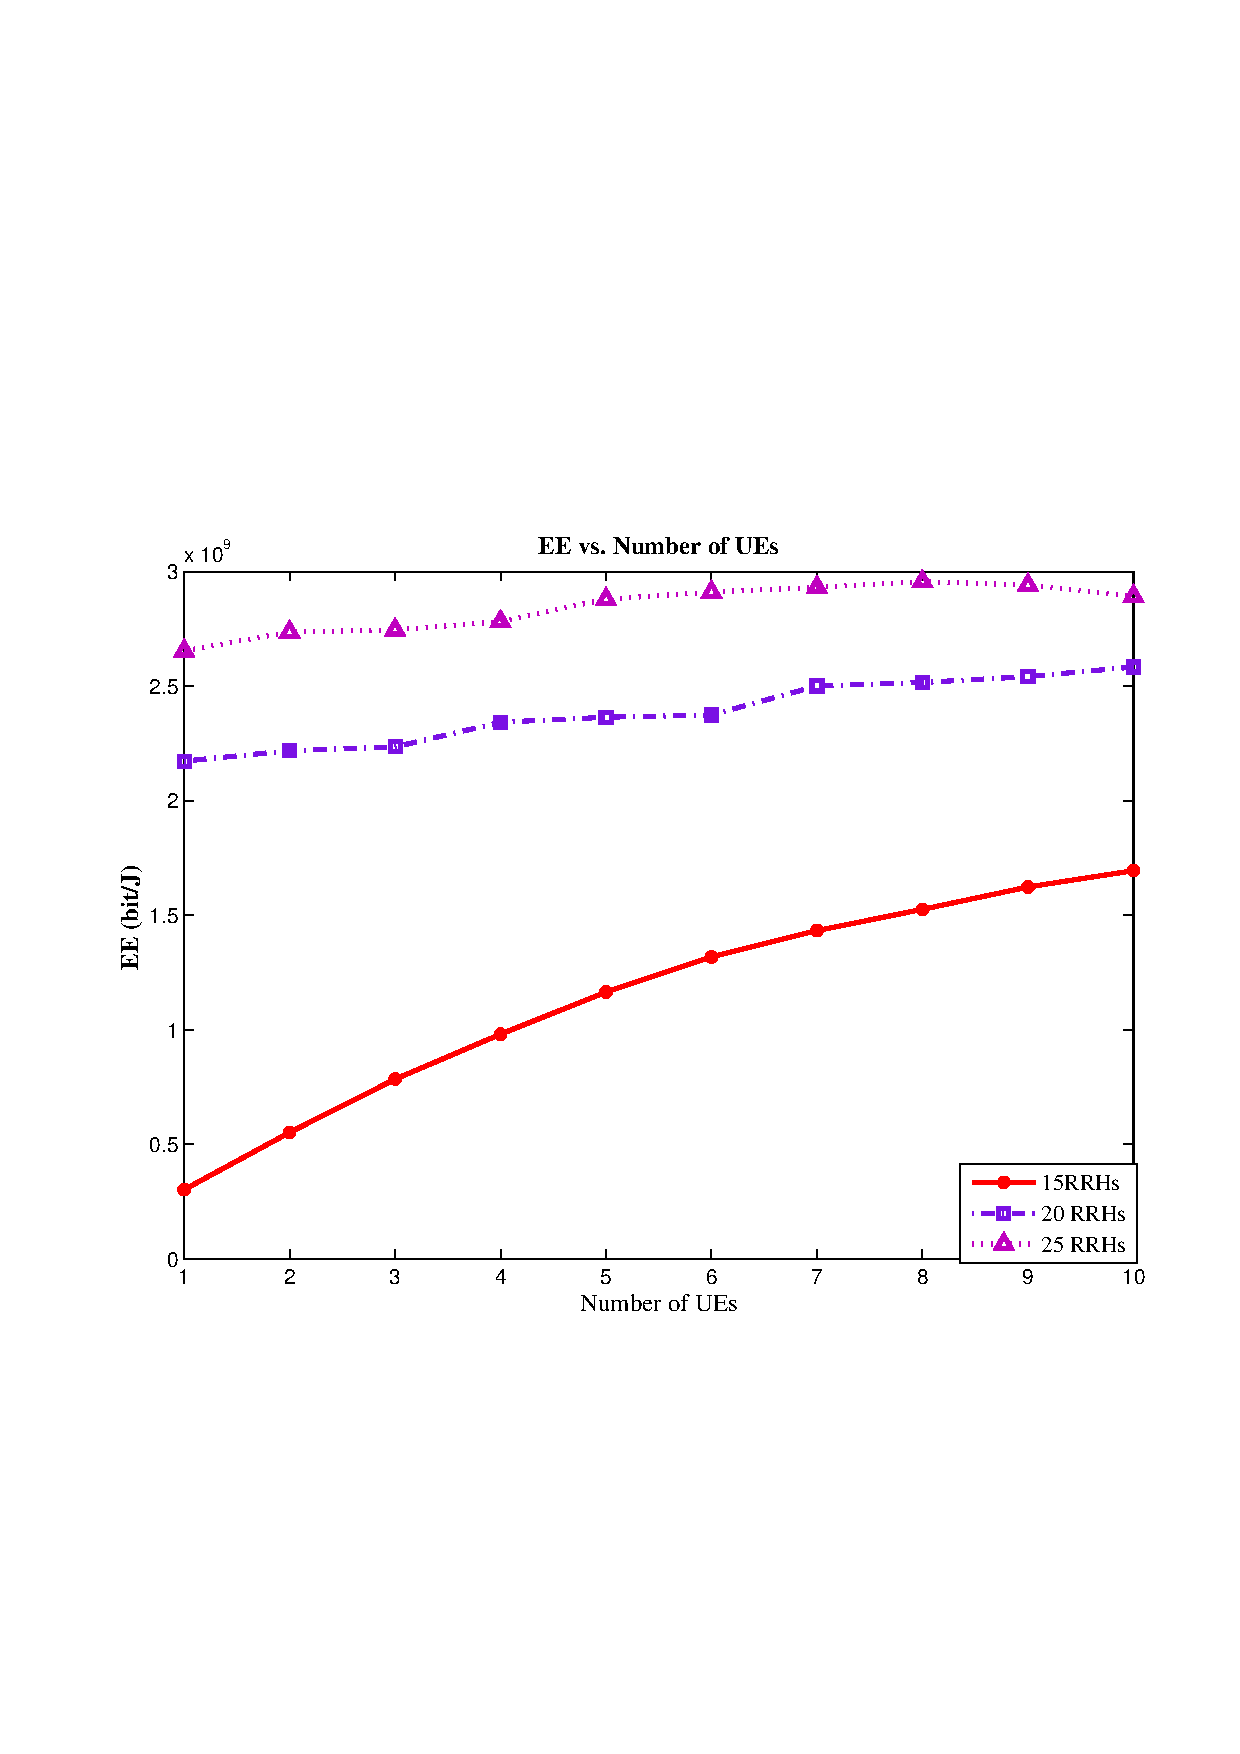
\includegraphics[width=\linewidth]{./fig/ue1}
  \caption{ٍ بازدهی انرژی برحسب تعداد کاربران برای یک خوشه برای
   3
   مقدار متفاوت واحد های رادیویی}
  \label{fig:ue1}
  \end{figure}
  در شکل \ref{fig:ue1}، بازدهی انرژی برحسب تعداد کاربران برای یک خوشه برای 3 مقدار متفاوت واحد های رادیویی با فرض $P_{max} = 10dbm$ رسم شده است. در این نمودار بیشینه ی ظرفیت محدود لینک \lr{fronthaul} مقدار 5 در نظر گرفته شده است و واریانس نویز کوانتیزاسیون $10^{-8}$ می باشد. با افزایش کاربران، بازدهی انرژی زیاد می گردد و  از جایی به بعد شیب افزایش آن رو به کاهش است که این کاهش به دلیل تداخل کاربران می باشد.
 
\begin{figure}[H]
  \centering
    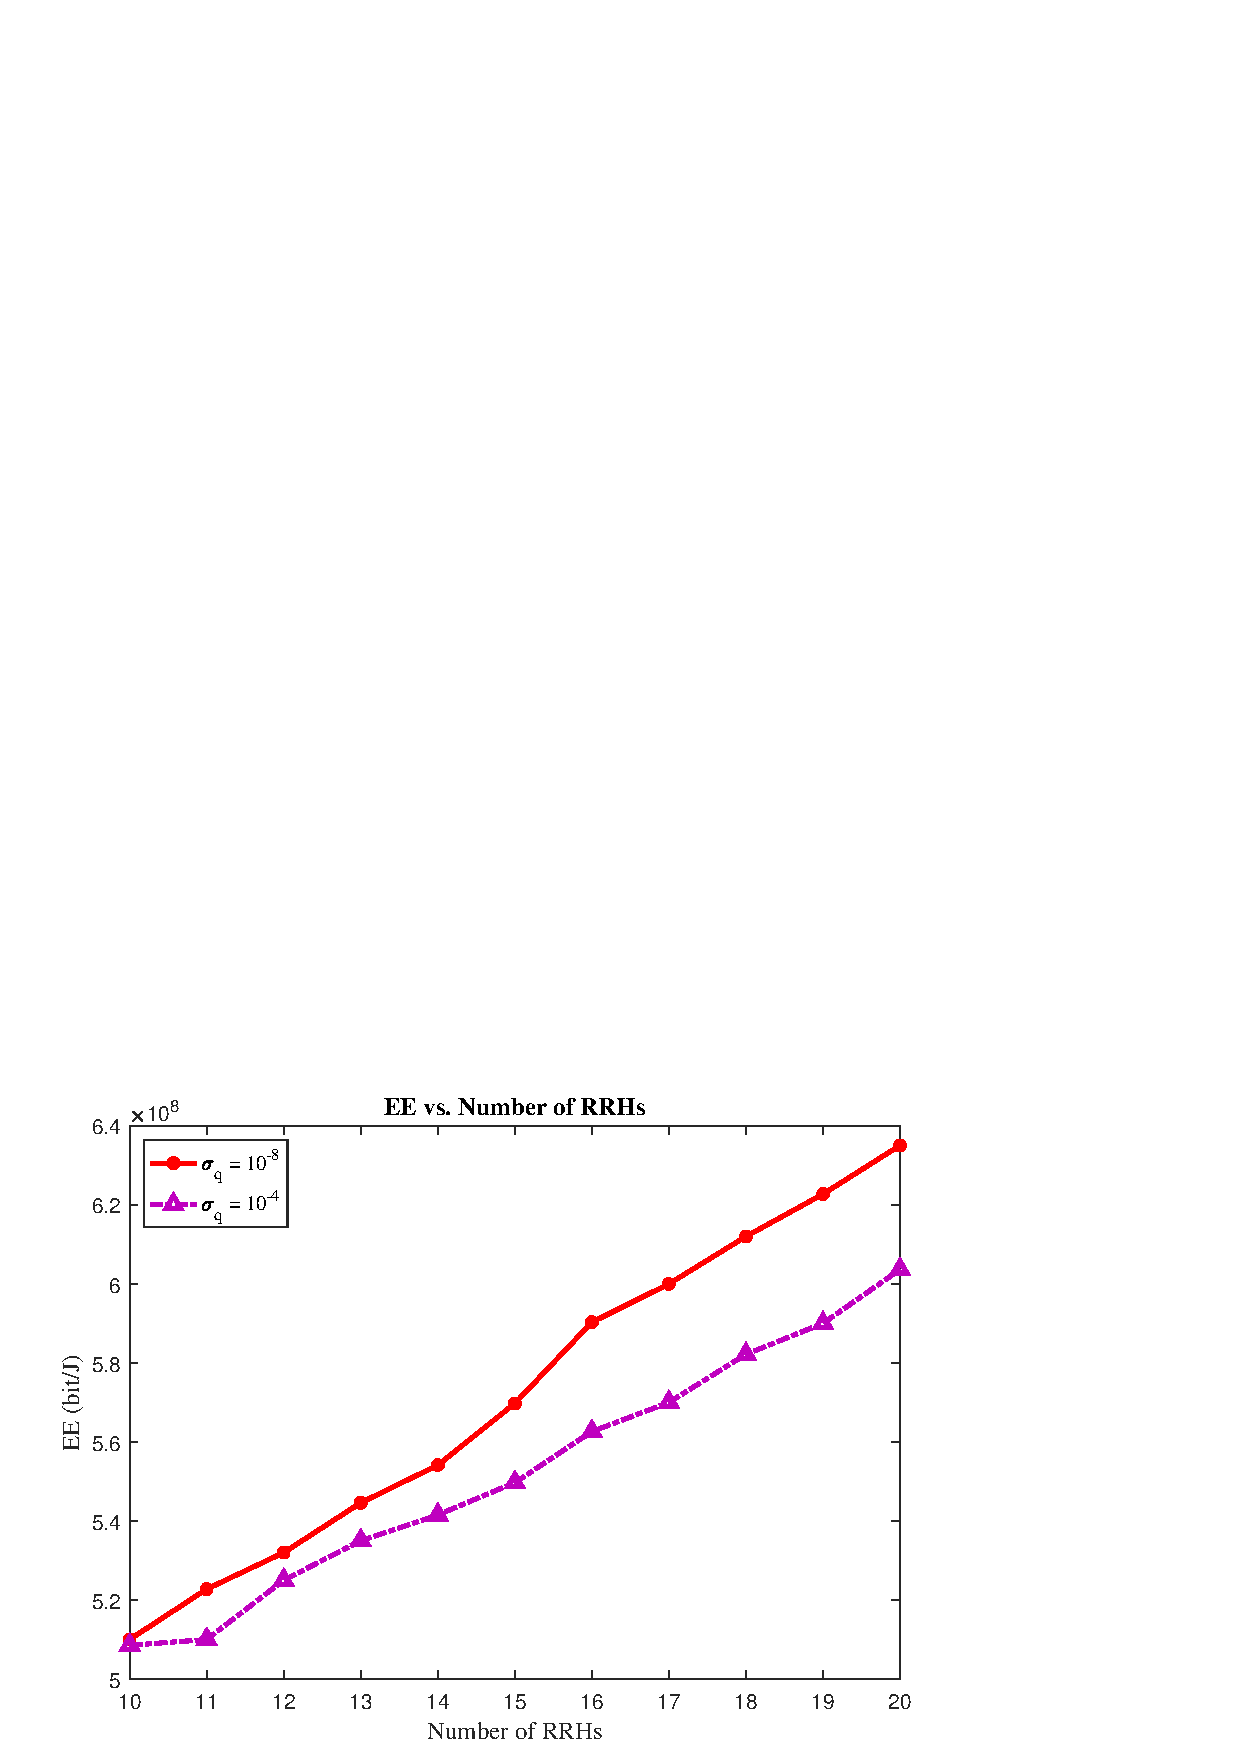
\includegraphics[width=\linewidth]{./fig/sigmaul}
  \caption{ٍ بازدهی انرژی برحسب تعداد واحدهای رادیویی برای2 کاربر  در دو حالت با نویز کوانتیزاسیون متفاوت }
  \label{fig:sigmaul}
  \end{figure}
      حال میزان بازدهی انرژی برحسب تعداد واحدهای رادیویی  در دو حالت با نویز کوانتیزاسیون متفاوت برای 2 کاربربا فرض های گفته شده برای شکل قبلی،  در شکل \ref{fig:sigmaul} ، رسم شده است.
  با توجه به شکل ، می توان فهمید که بازدهی انرژی برای زمانی که میزان نویز کمتر است بیشتر می باشد.
\subsection{مقایسه ی روش های بیان شده}
در این بخش، مدل سیستمهای مختلف در لینک فراسو با یکدیگر مقایسه می شوند.
درهردو مدل سیستم فشرده سازی و محدودیت لینک \lr{fronthaul} مورد بررسی قرار گرفته شده است. همچنین در هر دو فرض شده که خوشه بندی صورت نگرفته است. 

در مدل سیستم اول، سیگنال یادگیری کانال نیز در ابتدا ارسال می گردد تا بتوان کانال را تخمین زد. ولی در مدل سیستم دوم فرض بر این است که تخمین کانال از قبل صورت گرفته شده است و در مورد تخمین کانال صحبتی صورت نمی گیرد. همچنین در مدل سیستم دوم از ترکیب خطی 
\lr{MRC}\LTRfootnote{Maximum Ratio Combination}
برای بازیابی سیگنال استفاده می گردد که در مدل سیستم اول مورد بررسی قرار نمی گیرد.
در مدل سیستم اول، هدف ما، بیشینه سازی مجموع نرخهای قابل دسترس است در صورتی که در مدل سیستم دوم هدف بیشینه سازی بازدهی انرژی می باشد.

\section{سیستم مخابراتی \lr{D2D} }
\subsection{مقدمه}
در این بخش مدل سیستم دیگری بیان می شود که دارای سیستم مخابراتی \lr{D2D} 
\LTRfootnote{Device-to-Device}
 می باشد \cite{d2d, d2dd} . سیستم \lr{D2D} منجر می شود که ساختار \lr{C-RAN} بازدهی طیفی بیشتر و تاخیر کمتری داشته باشد. در حال حاضر، تحقیقات زیادی در زمینه ی تخصیص منابع برای سیستم های مخابراتی \lr{D2D} صورت گرفته است.
 حال در اینجا این مدل سیستم در ساختار \lr{C-RAN} بررسی می شود \cite{rd2d}.
 \subsection{مدل سیستم}
  در این ساختار، شبکه دارای $N$ تا واحد رادیویی یا \lr{RRH} $M$ آنتنه می باشد. همچنین این ساختار دارای $K$ جفت کاربر \lr{D2D} تک آنتنه می باشد که در هر جفت یکی فرستنده است که با $T_x$ نمایش داده می شود و دیگری گیرنده می باشد که با $R_x$ نمایش می دهیم. 
علاوه بر این فرض می شود واحد کنترل یا \lr{BBU pool} به خوبی می تواند کانال را تخمین بزند. 
همچنین این مدل سیستم در دو وضعیت \lr{C-RAN} و \lr{D2D} کار می کند که در بازه های زمانی مختلف در وضعیت های مختلف عمل می کند. 
فرض کنید در بازه ی زمانی  
$[t,t+1)$
سیگنال ارسالی از $k$ امین کاربر فرستنده ی  
$T_x$
، در وضعیت \lr{C-RAN} به صورت مقابل می باشد
\begin{equation}
\begin{split}
y^C_k(t) =& \sum_{n=1}^{N} \boldsymbol{v}_{n,k}^{H}(t) \boldsymbol{g}_{n,k}^{C}(t) \sqrt{p_k(t)} s_k(t) \\
+& \sum_{n=1}^{N} \sum_{l\neq k}^{K} \boldsymbol{v}_{n,k}^{H}(t) \boldsymbol{g}_{n,l}^{C}(t) \sqrt{p_l(t)} s_l(t) \\
+& \sum_{n=1}^{N} \boldsymbol{v}_{n,k}^{H}(t) \boldsymbol{z}_n(t)
\end{split}
\end{equation}
 که در اینجا، $\boldsymbol{v}_{n,k} \in \mathsf{C}^{M\times 1}$
  نشان دهنده ی بردار پرتو دهی بین
 کاربر $k$ ام  و  واحد رادیویی $n$ ام می باشد.

می باشد. 
 همچنین 
 $\boldsymbol{g}_{n,k}^{C}(t) \in \mathsf{C}^{M\times 1}$
 بردار کانال بین  کاربر $k$ ام  و  واحد رادیویی $n$ ام است.  
 $\boldsymbol{z}_n(t) \backsim \mathcal{N}(0,\sigma^2 \boldsymbol{I}_M )$
 نیز، بردار نویز گوسی است.
علاوه بر این، $p_k(t)$ و $s_k(t)$ به ترتیب نشان دهنده ی توان ارسالی و سیگنال ارسالی از کاربر $k$  می باشد. 
 در این وضعیت، نرخ قابل دسترس از رابطه ی زیر بدست می آید:
\begin{equation}
R^{C}_k(t) = \log_2(1+ \frac{p_k(t) |\boldsymbol{v}_{k}^{H}(t) \boldsymbol{g}_{k}^{C}(t)|^2 }{ \sum_{l\neq k}^{K}p_l(t) |\boldsymbol{v}_{k}^{H}(t) \boldsymbol{g}_{l}^{C}(t)|^2 + \sigma^2 || \boldsymbol{v}_{k}||^2_2})
\end{equation}
که در اینجا،$\boldsymbol{v}_{k} \in \mathsf{C}^{NM\times 1}$ بردار پرتودهی برای کاربر $k$ می باشد
که به صورت \\
 $\boldsymbol{v}_{k}^{C}(t) = [{\boldsymbol{v}_{1,k}^{C}(t)}^T, ... , {\boldsymbol{v}_{N,k}^{C}(t)}^T ]^T$
است. 
 همچنین 
 $\boldsymbol{g}_{k}^{C}(t) \in \mathsf{C}^{NM \times 1}$
 بردار کانال بین کاربر $k$ام و واحدهای رادیویی است.\newline
  که به صورت 
  $\boldsymbol{g}_{k}^{C}(t) = [{\boldsymbol{g}_{1,k}^{C}(t)}^T, ... , {\boldsymbol{g}_{N,k}^{C}(t)}^T ]^T$
 می باشد.
 به صورت مشابه، سیگنال دریافتی توسط کاربر $R_x$ در حالت \lr{D2D} به صورت مقابل می باشد:

\begin{equation}
y^D_i(t) =  {g}_{i,i}^{D}(t) \sqrt{p_i(t)} s_i(t) 
+ \sum_{j\neq i}^{K} {g}_{j,i}^{D}(t) \sqrt{p_j(t)} s_j(t) + \phi_i(t) 
\end{equation}
که در اینجا  
$ \boldsymbol{g}_{i,i}^{D}$
بردار کانال بین $i$ امین جفت فرستنده و گیرنده ی \lr{D2D} می باشند. همچنین 
 $\phi_i(t) \backsim \mathcal{N}(0,\sigma^2 )$
 نویز گوسی است.\newline
 نرخ قابل دسترس 
 در اینجا از رابطه ی زیر بدست می آید:
 \begin{equation}
R^{D}_k(t) = \log_{2} (1+ \frac{p_i(t) |g_{i,i}^{D}(t)|^2 }{ \sum_{j\neq i}^{K} p_j(t) |g_{j,i}^D (t)|^2 + \sigma^2 })
\end{equation}
برای انتخاب وضعیت های متفاوت در بازه ی زمانی $t$  برای جفت کاربر$k$ از رابطه ی زیر استفاده می شود.
%\begin{equation}
\begin{latin}
\[ 
x_k(t) =
\left \{
 \begin{tabular}{cc}
  0,  & \text{\lr{C-RAN mode}} \\
  1,  & \text{\lr{D2D mode}} \\
  \end{tabular}
  \right \}
\]
%\end{equation}
\end{latin}
بنابراین با توجه به  رابطه ی بالا نرخ قابل دسترس  برای  $k$ امین جفت کاربر به صورت زیر بدست می آید:
\begin{equation}
R_k(t)  = (1-x_k(t)) R_k^C(t) + x_k(t) R_k^D(t)
\end{equation}
میانگین نرخ قابل دسترس برای $k$ امین جفت \lr{D2D} از رابطه ی مقابل بدست می آید:
\begin{equation}
\bar{R_k} = \lim_{T\to\infty} \frac{1}{T} \sum_{t=0}^{T-1} \mathrm{E}\{R_k(t)\} 
\end{equation}
حال در اینجا هدف، بیشینه سازی مجموع میانگین نرخ قابل دسترس با شروطی که بیان می گردد، می باشد که در ادامه نمایش داده شده است.
   \begin{equation}
\begin{aligned}
\max\limits_{\boldsymbol{p}(t),  \boldsymbol{x}(t)}   \quad &   \sum_{k=1}^{K}(\bar{R_k})\\
\text{\lr{subject to}} \quad  &  0 \leq {p}_{k} \leq P_{max} && \qquad \forall k,   \\
& \sum_{k=1}^{K} x_k(t) p_k(t) \ P_{max}^{k} && \qquad \forall k, \\ 
&x_k(t) \in \{ 0, 1 \}  &&\qquad  \forall ik\\
\end{aligned}			
\end{equation}
\section{نتیجه گیری}
در این فصل ابتدا لینک فروسو و سپس لینک فراسو را مورد بررسی قرارگرفته است. در لینک فروسو سه مدل سیستم متفاوت بررسی شده اند که در فصل بعدی دو مدل سیستم اول را با یکدیگر ادغام کرده و مدل سیستم جدیدی بیان می شود. همچنین در لینک فراسو نیز دو مدل سیستم متفادت بیان شده است که در ادامه ی فصل سوم مدل سیستمی شامل چندین خوشه به همراه لینک محدود \lr{fronthaul} تعریف می شود. در قسمت آخر این فصل، مدل سیستم \lr{D2D} معرفی شده که در حال حاضر می توان در این زمینه، کارهای نوینی انجام داد. 
